\section*{Results}
\subsection{RSTF directivity}
\begin{itemize}
    \item RSTF deconvolution for both 2015 and 2025 earthquakes are performed on the data of the worldwide broadband sations shown
     in the Figure~\ref{fig:2015_station} and Figure~\ref{fig:2025_station}.
    \item  Figure~\ref{fig:2015_rstf} and Figure~\ref{fig:2025_rstf} 
     represent relative source time functions (RSTFs)
      at these stations obtained by the Projected Landweber Method \cite{RSTFVallée2004}.
    \item The RSTFs (Fiugure~\ref{fig:2015_rstf} and Figure~\ref{fig:2025_rstf}) show a clear azimuthal dependence, with a stretched profile toward the east and a compressed profile toward
     the west. This pattern is consistent with the directivity effect caused by rupture propagation from west to east
      \cite{Aderhold2016}. The same pattern is observed for both the 2015 and 2025 earthquakes, suggesting that the two events
       had a similar rupture propagation direction.
    \item However, the RSTFs for the 2025 earthquake show stronger stretching and compression compared to those of the 2015 earthquake.
     This suggests that the 2025 rupture was more spatially distributed and lasted longer than the 2015 rupture. This is also 
     consistent with the longer rupture duration estimated for the 2025 earthquake shown in Figure.
\end{itemize}

\begin{figure}[H]
    \centering

    \resizebox{0.6\textwidth}{!}{
        \begin{minipage}{\textwidth}
            \centering
            % ---------- 2015 ----------
            \begin{subfigure}{0.5\textwidth}
           
                \centering
                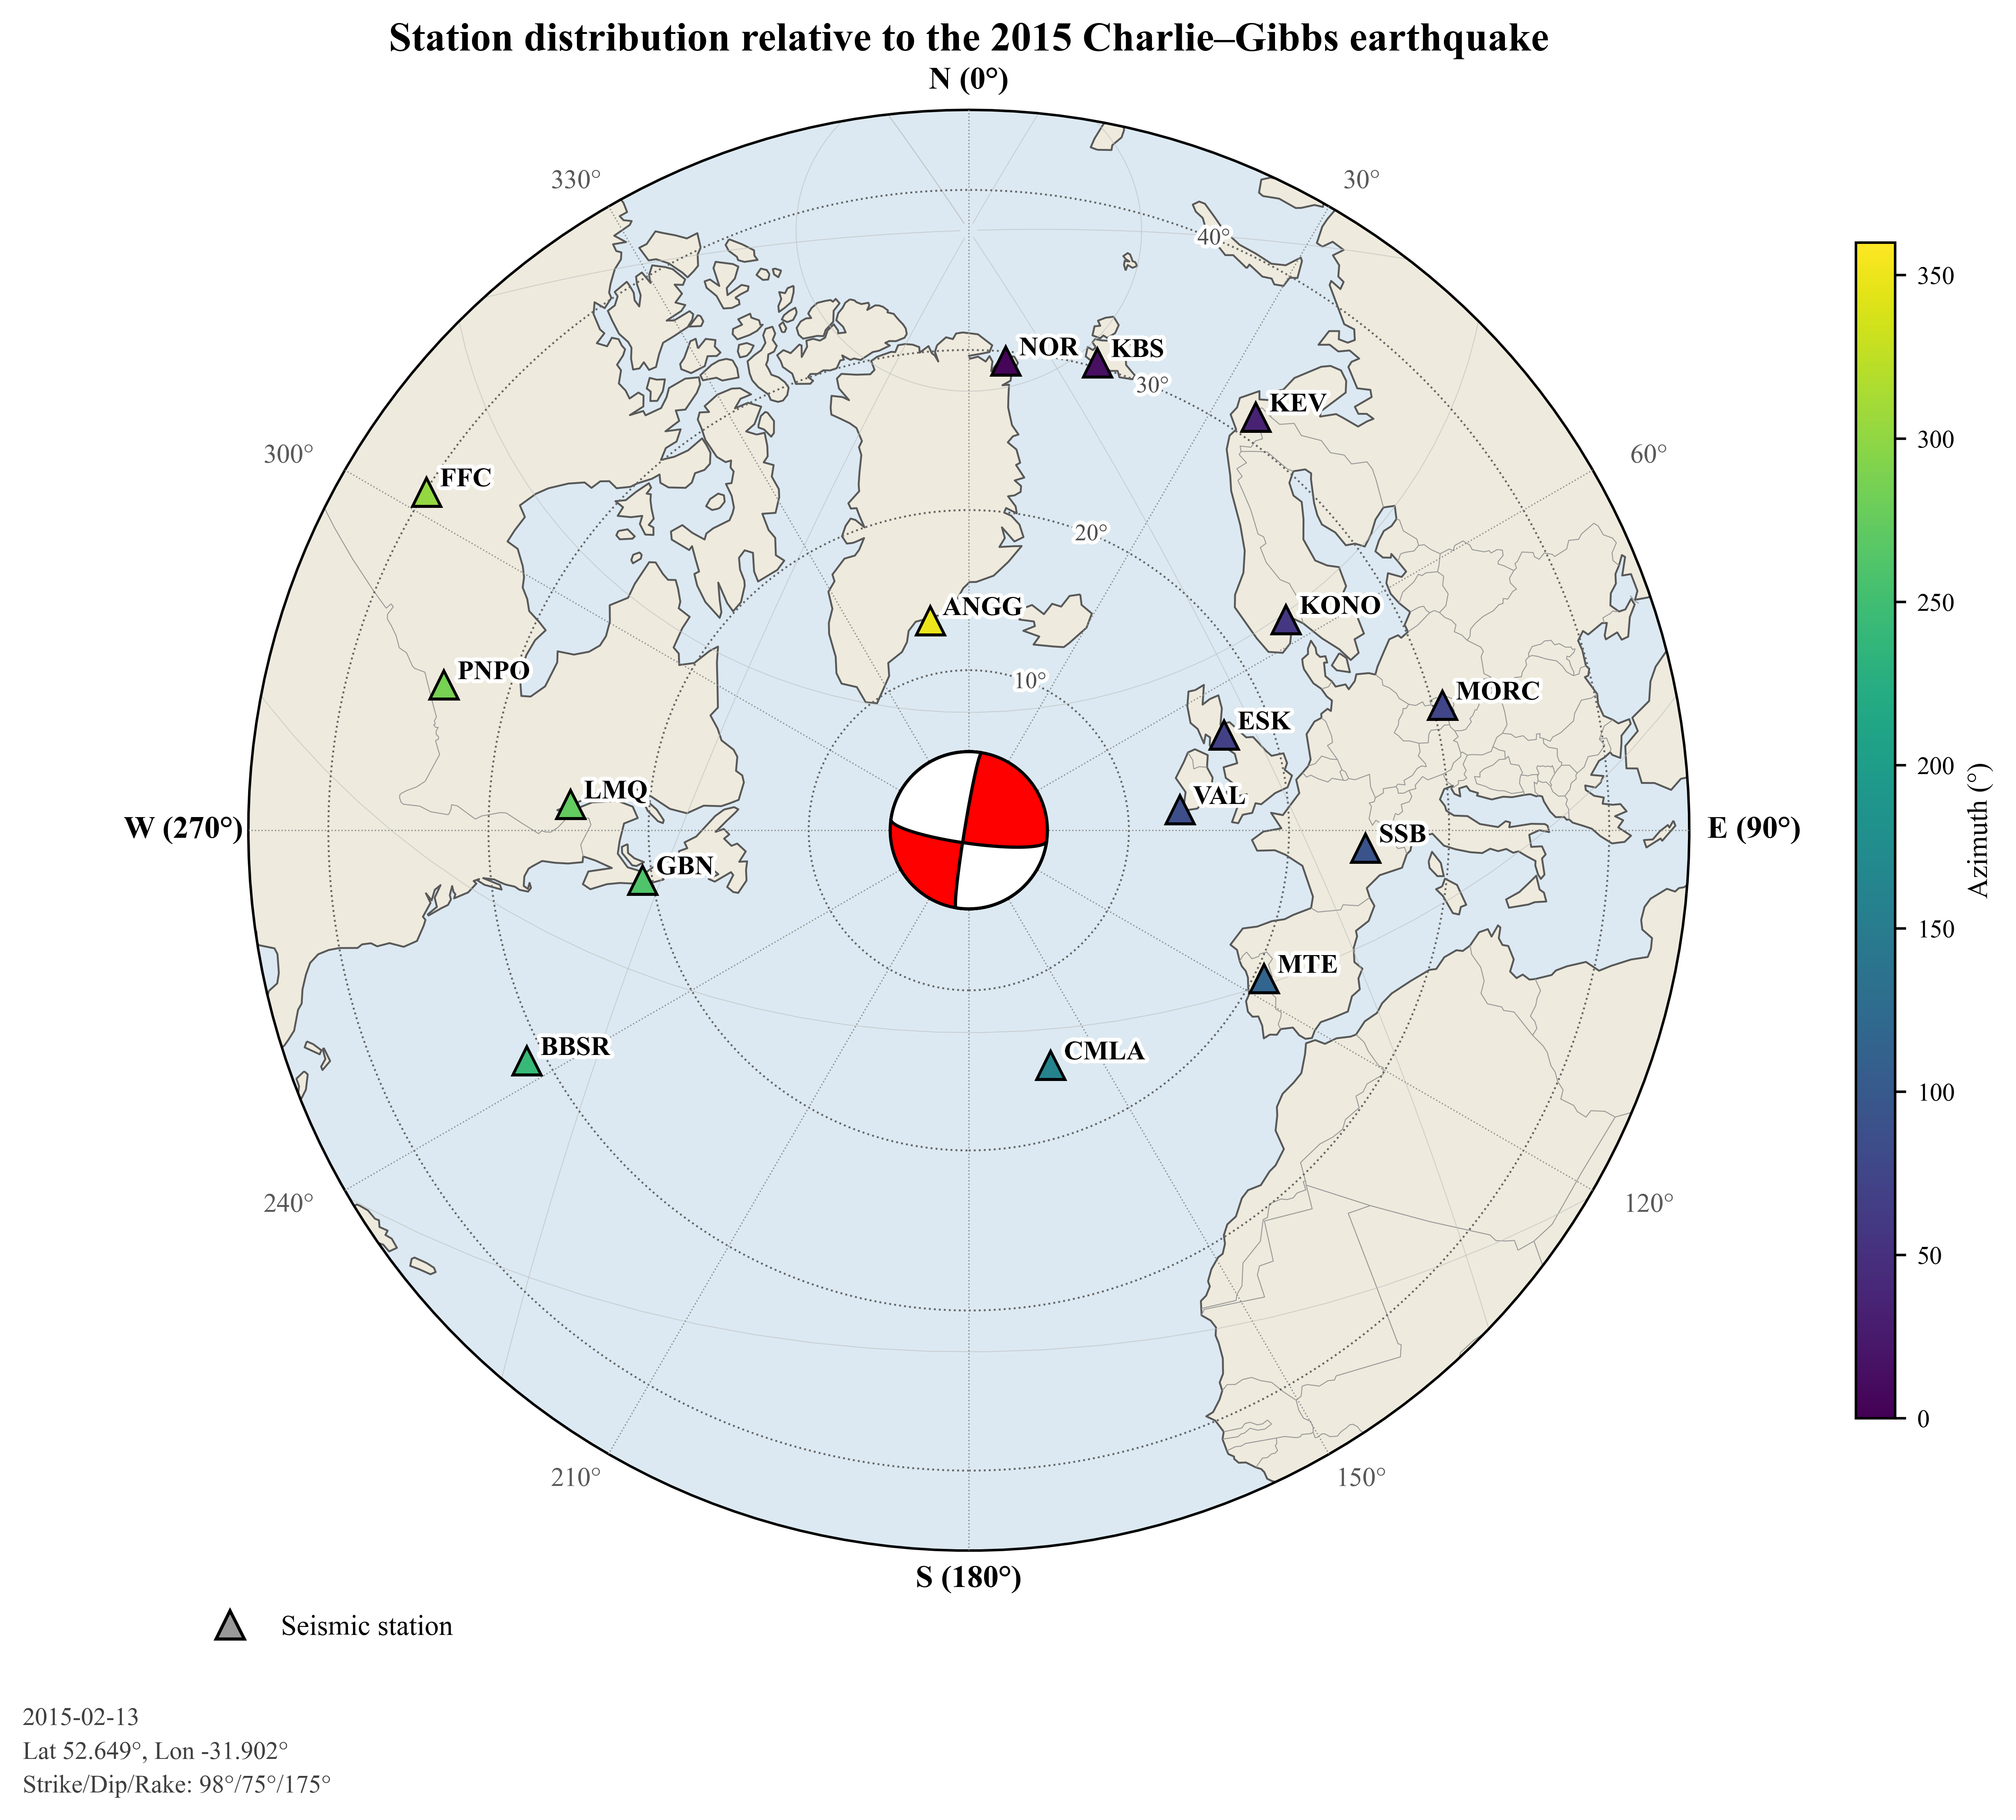
\includegraphics[width=\textwidth]{diagrams/2015_Charlie_Gibbs_station_distribution_focal_mechanism.png}
                \caption{}
                \label{fig:2015_station}
            \end{subfigure}
            \hfill
            \begin{subfigure}{0.4\textwidth}
                \centering
                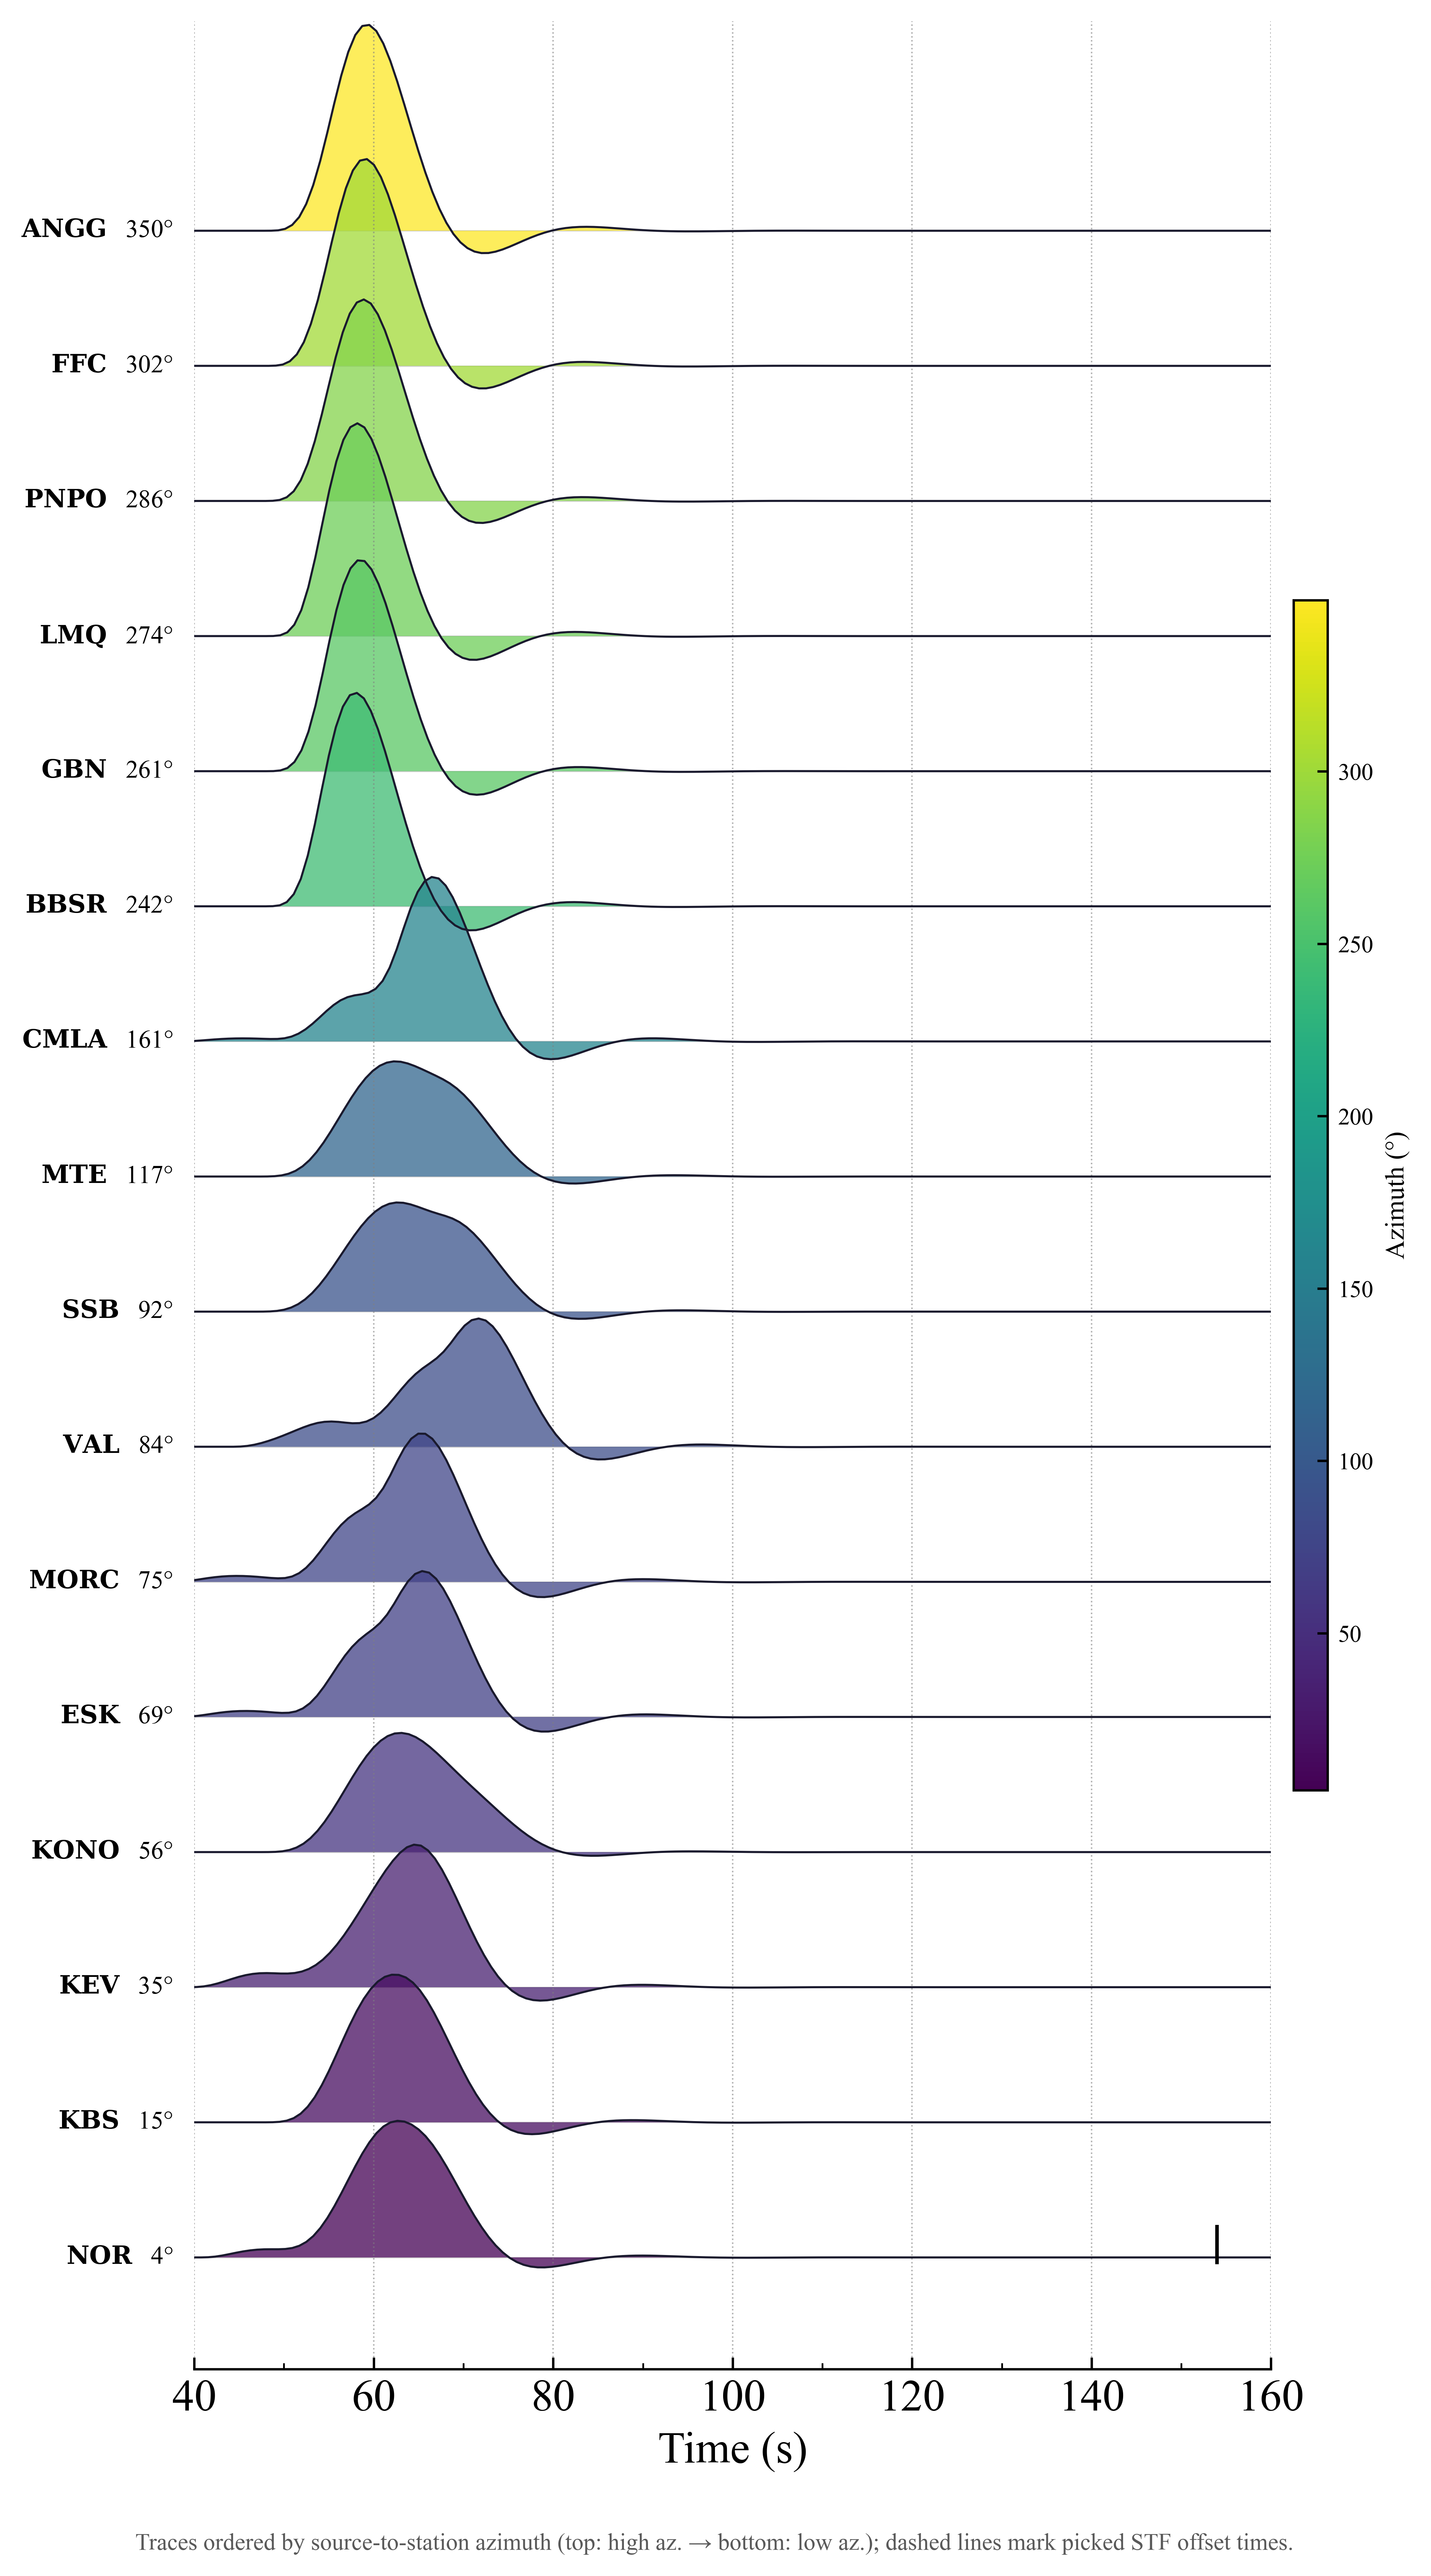
\includegraphics[width=\textwidth]{diagrams/2015_RSTF_azimuthal.png}
                \caption{}
                \label{fig:2015_rstf}
            \end{subfigure}

            \vspace{0.1cm}

            % ---------- 2025 ----------
            \begin{subfigure}{0.5\textwidth}
                \centering
                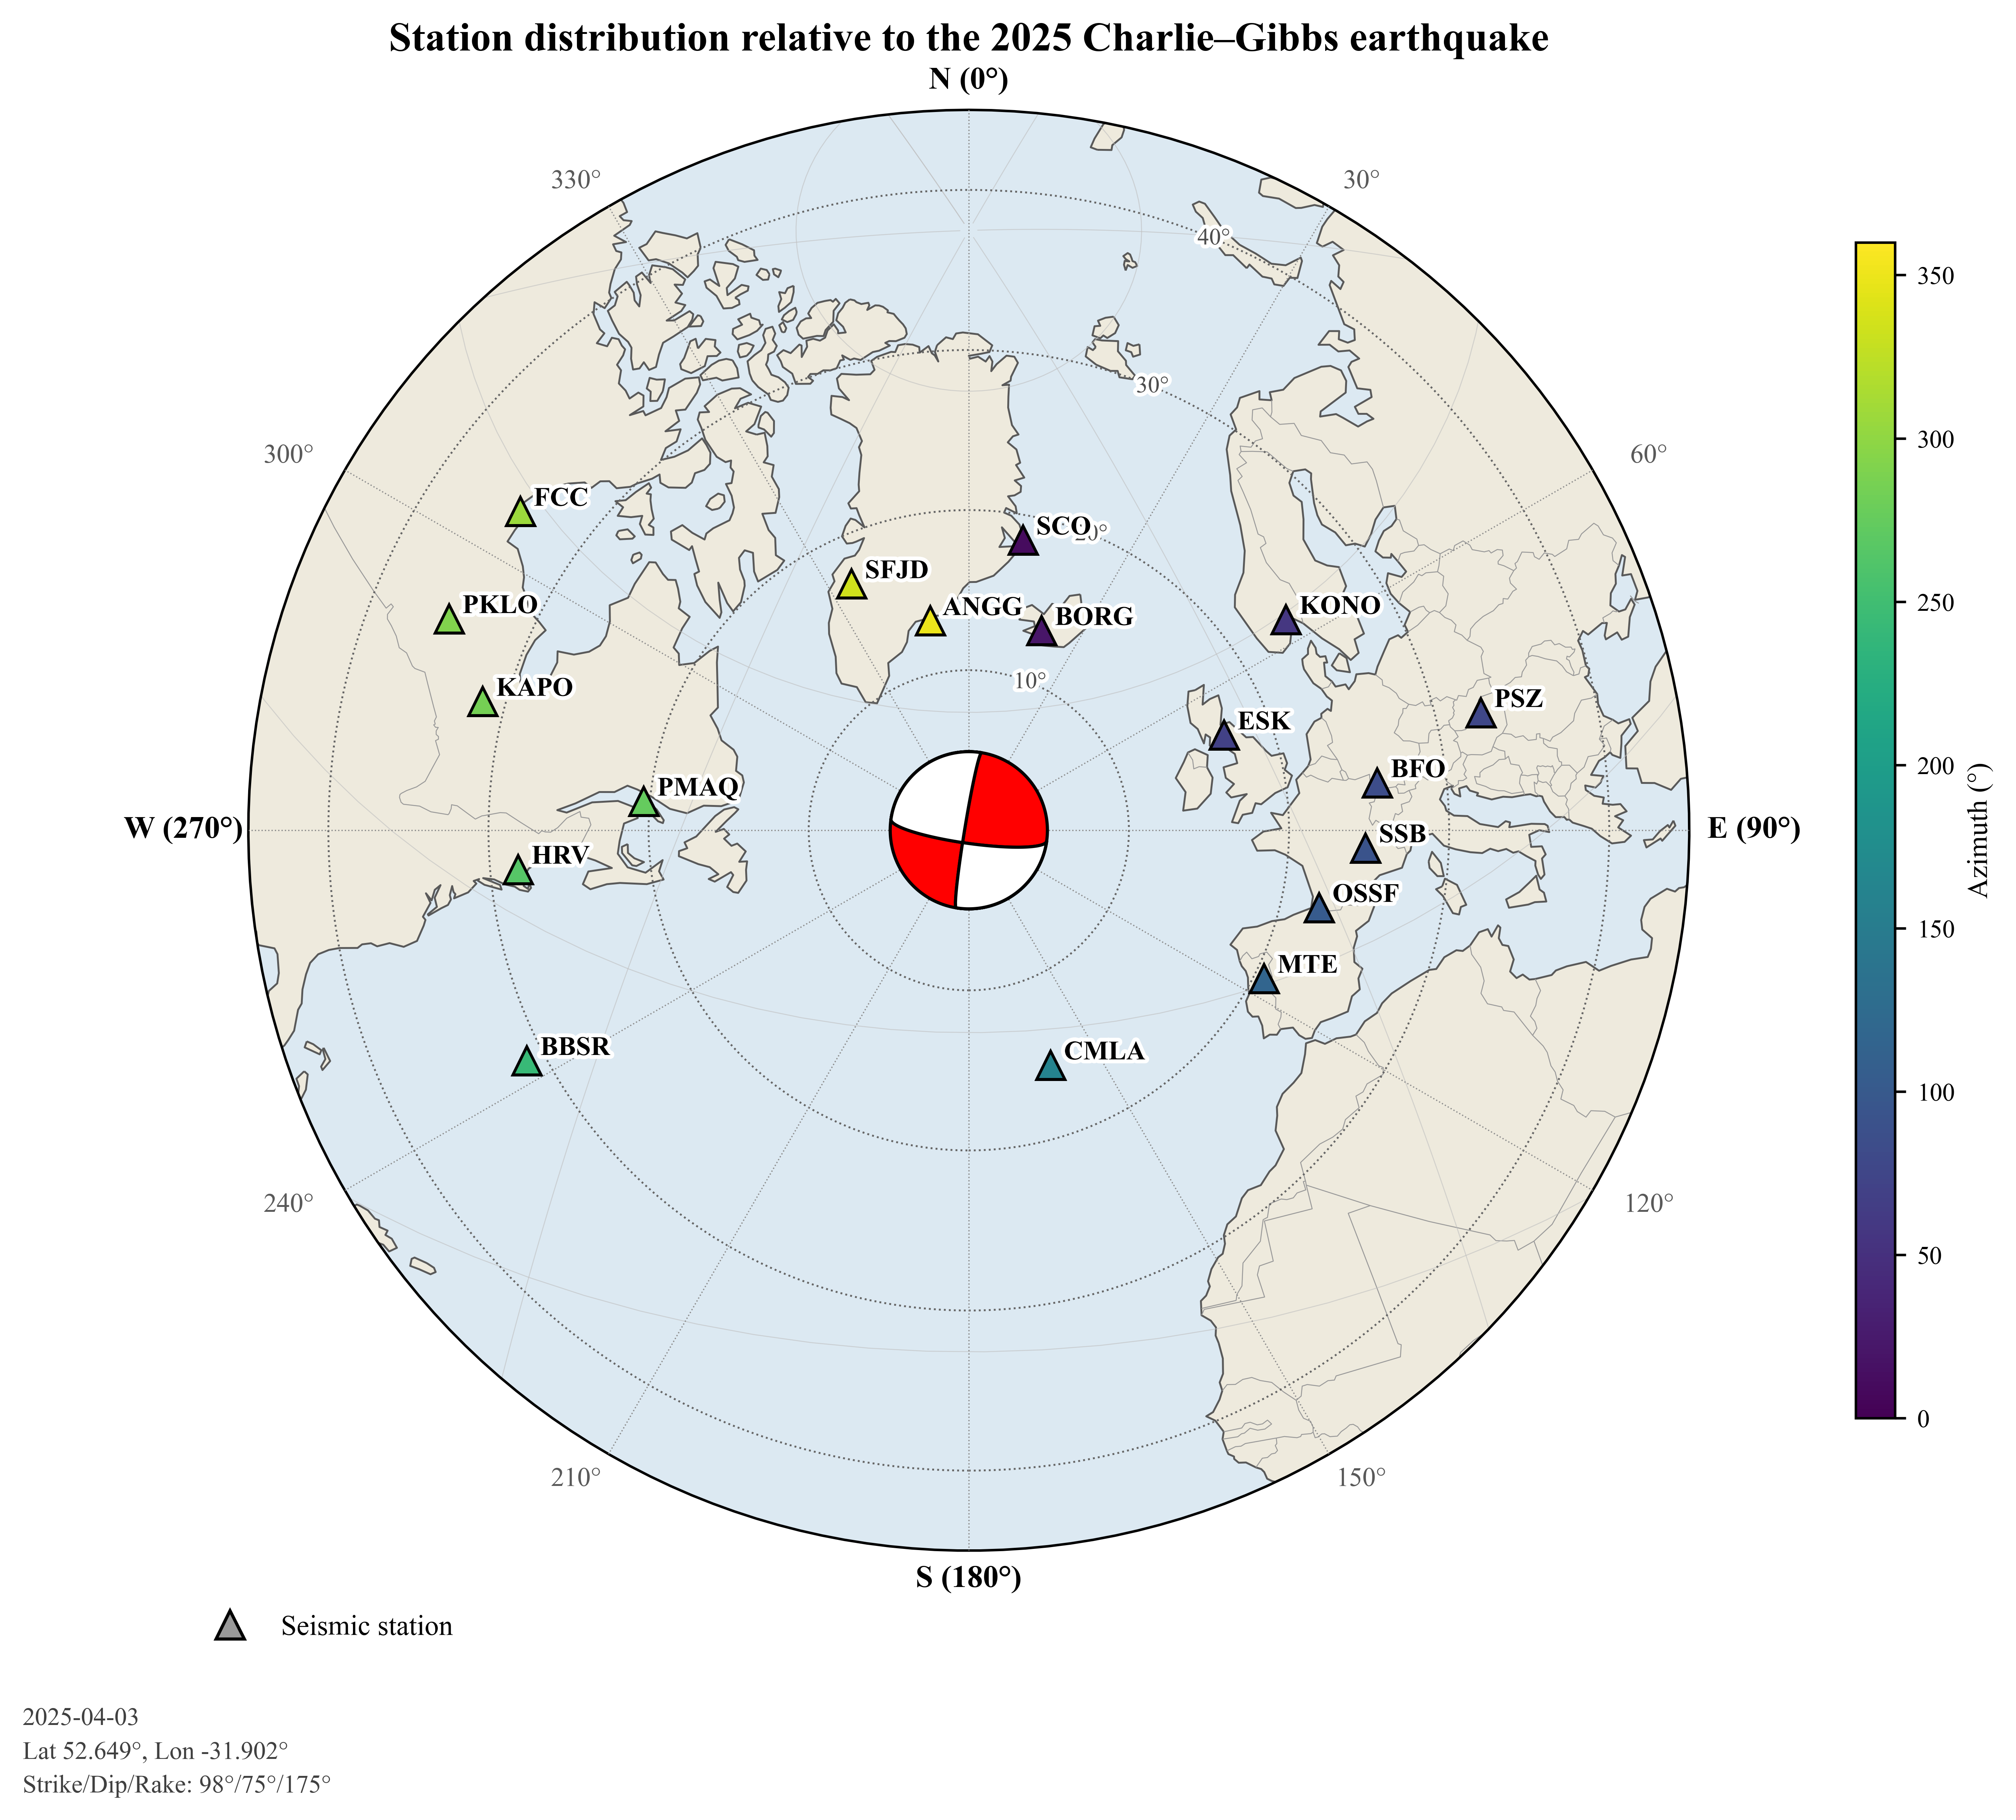
\includegraphics[width=\textwidth]{diagrams/2025_Charlie_Gibbs_station_distribution_focal_mechanism.png}
                \caption{}
                \label{fig:2025_station}
            \end{subfigure}
            \hfill
            \begin{subfigure}{0.4\textwidth}
                \centering
                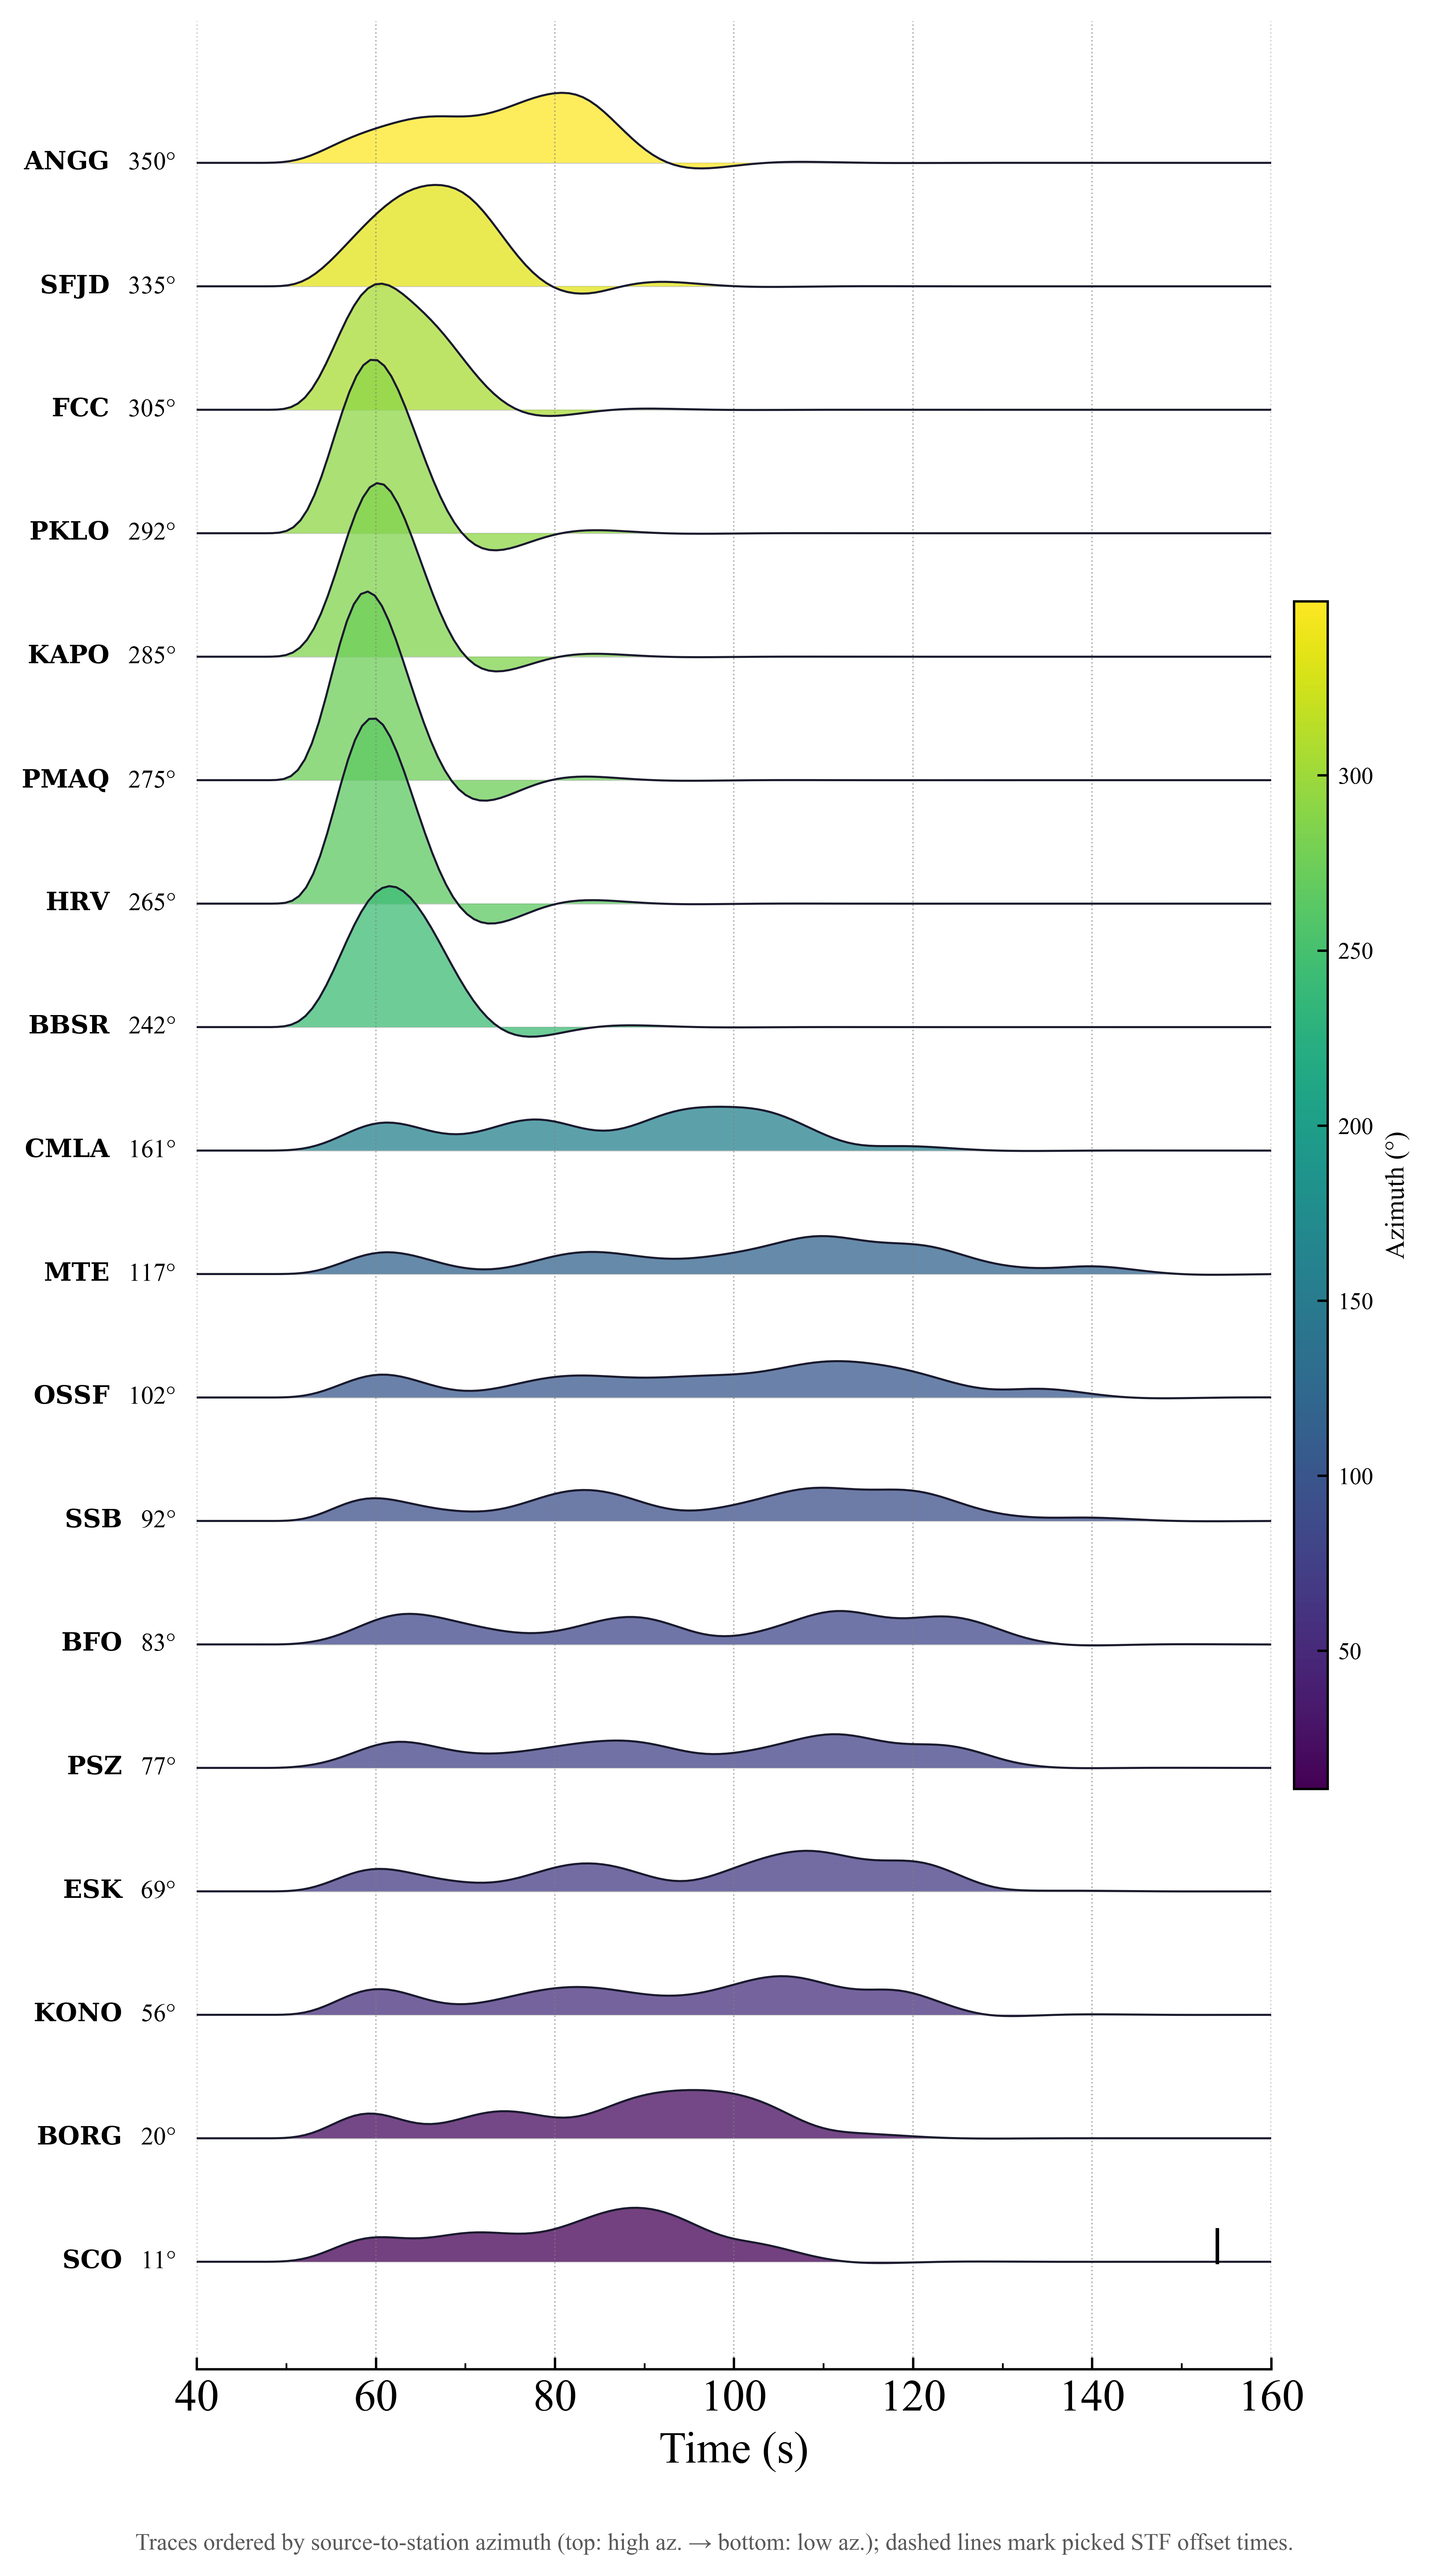
\includegraphics[width=\textwidth]{diagrams/2025_RSTF_azimuthal.png}
                \caption{}
                \label{fig:2025_rstf}
            \end{subfigure}
        \end{minipage}
    
    }
    \caption{Relative source time functions (RSTFs) from Love wave analysis (Projected Landweber Method) and station
     distributions for the 2015 and 2025 Charlie--Gibbs earthquakes. (a) Station distribution used for the determination of RSTFs 
     for the 2015 earthquake. Triangles denote broadband stations, the red focal mechanism indicates the earthquake source, and 
     concentric circles show epicentral distance. Station colors correspond to epicentral distance. (b) RSTFs for the 2015 earthquake
     plotted as a function of station azimuth. The systematic variation in RSTF shape and duration with azimuth indicates a clear
     azimuthal dependence of the apparent source duration. (c) Station distribution and focal mechanism for the 2025 earthquake,
     shown using the same convention as in (a). (d) Azimuthal distribution of RSTFs for the 2025 earthquake. Compared with 2015,
     the 2025 RSTFs exhibit more pronounced stretching and compression with azimuth, consistent with its longer source duration.}

    \label{fig:2015_2025_comparison}

\end{figure}
\end{itemize}
\subsection{Joint inversion results}
\begin{itemize}[label=--,itemsep=2pt, topsep=0pt]
    \item The fault slip distribution inversion is based on the analysis of the worldwise broadand teleseismic
     P- and S-wave data 
    shown in Figure~\ref{fig:2015_tele_station} and Figure~\ref{fig:2025_tele_station}.
    \item Using the same fault geometry for both earthquakes, we inverted for the fault slip distribution. The resulting models 

    show good agreement between the observed and predicted teleseismic waveforms for both events, as shown in 
    Figure~\ref{fig:2015_tele_inversion} and Figure~\ref{fig:2025_tele_inversion}. The aggregate RMS misfit is 0.394 for the 2015 
    earthquake and 0.453 for the 2025 earthquake.
\begin{figure}[H]
    \centering

    \resizebox{0.8\textwidth}{!}{%
        \begin{minipage}{\textwidth}
            \centering

            % ---------- 2015 ----------
            \begin{subfigure}{0.40\textwidth}
                \centering
                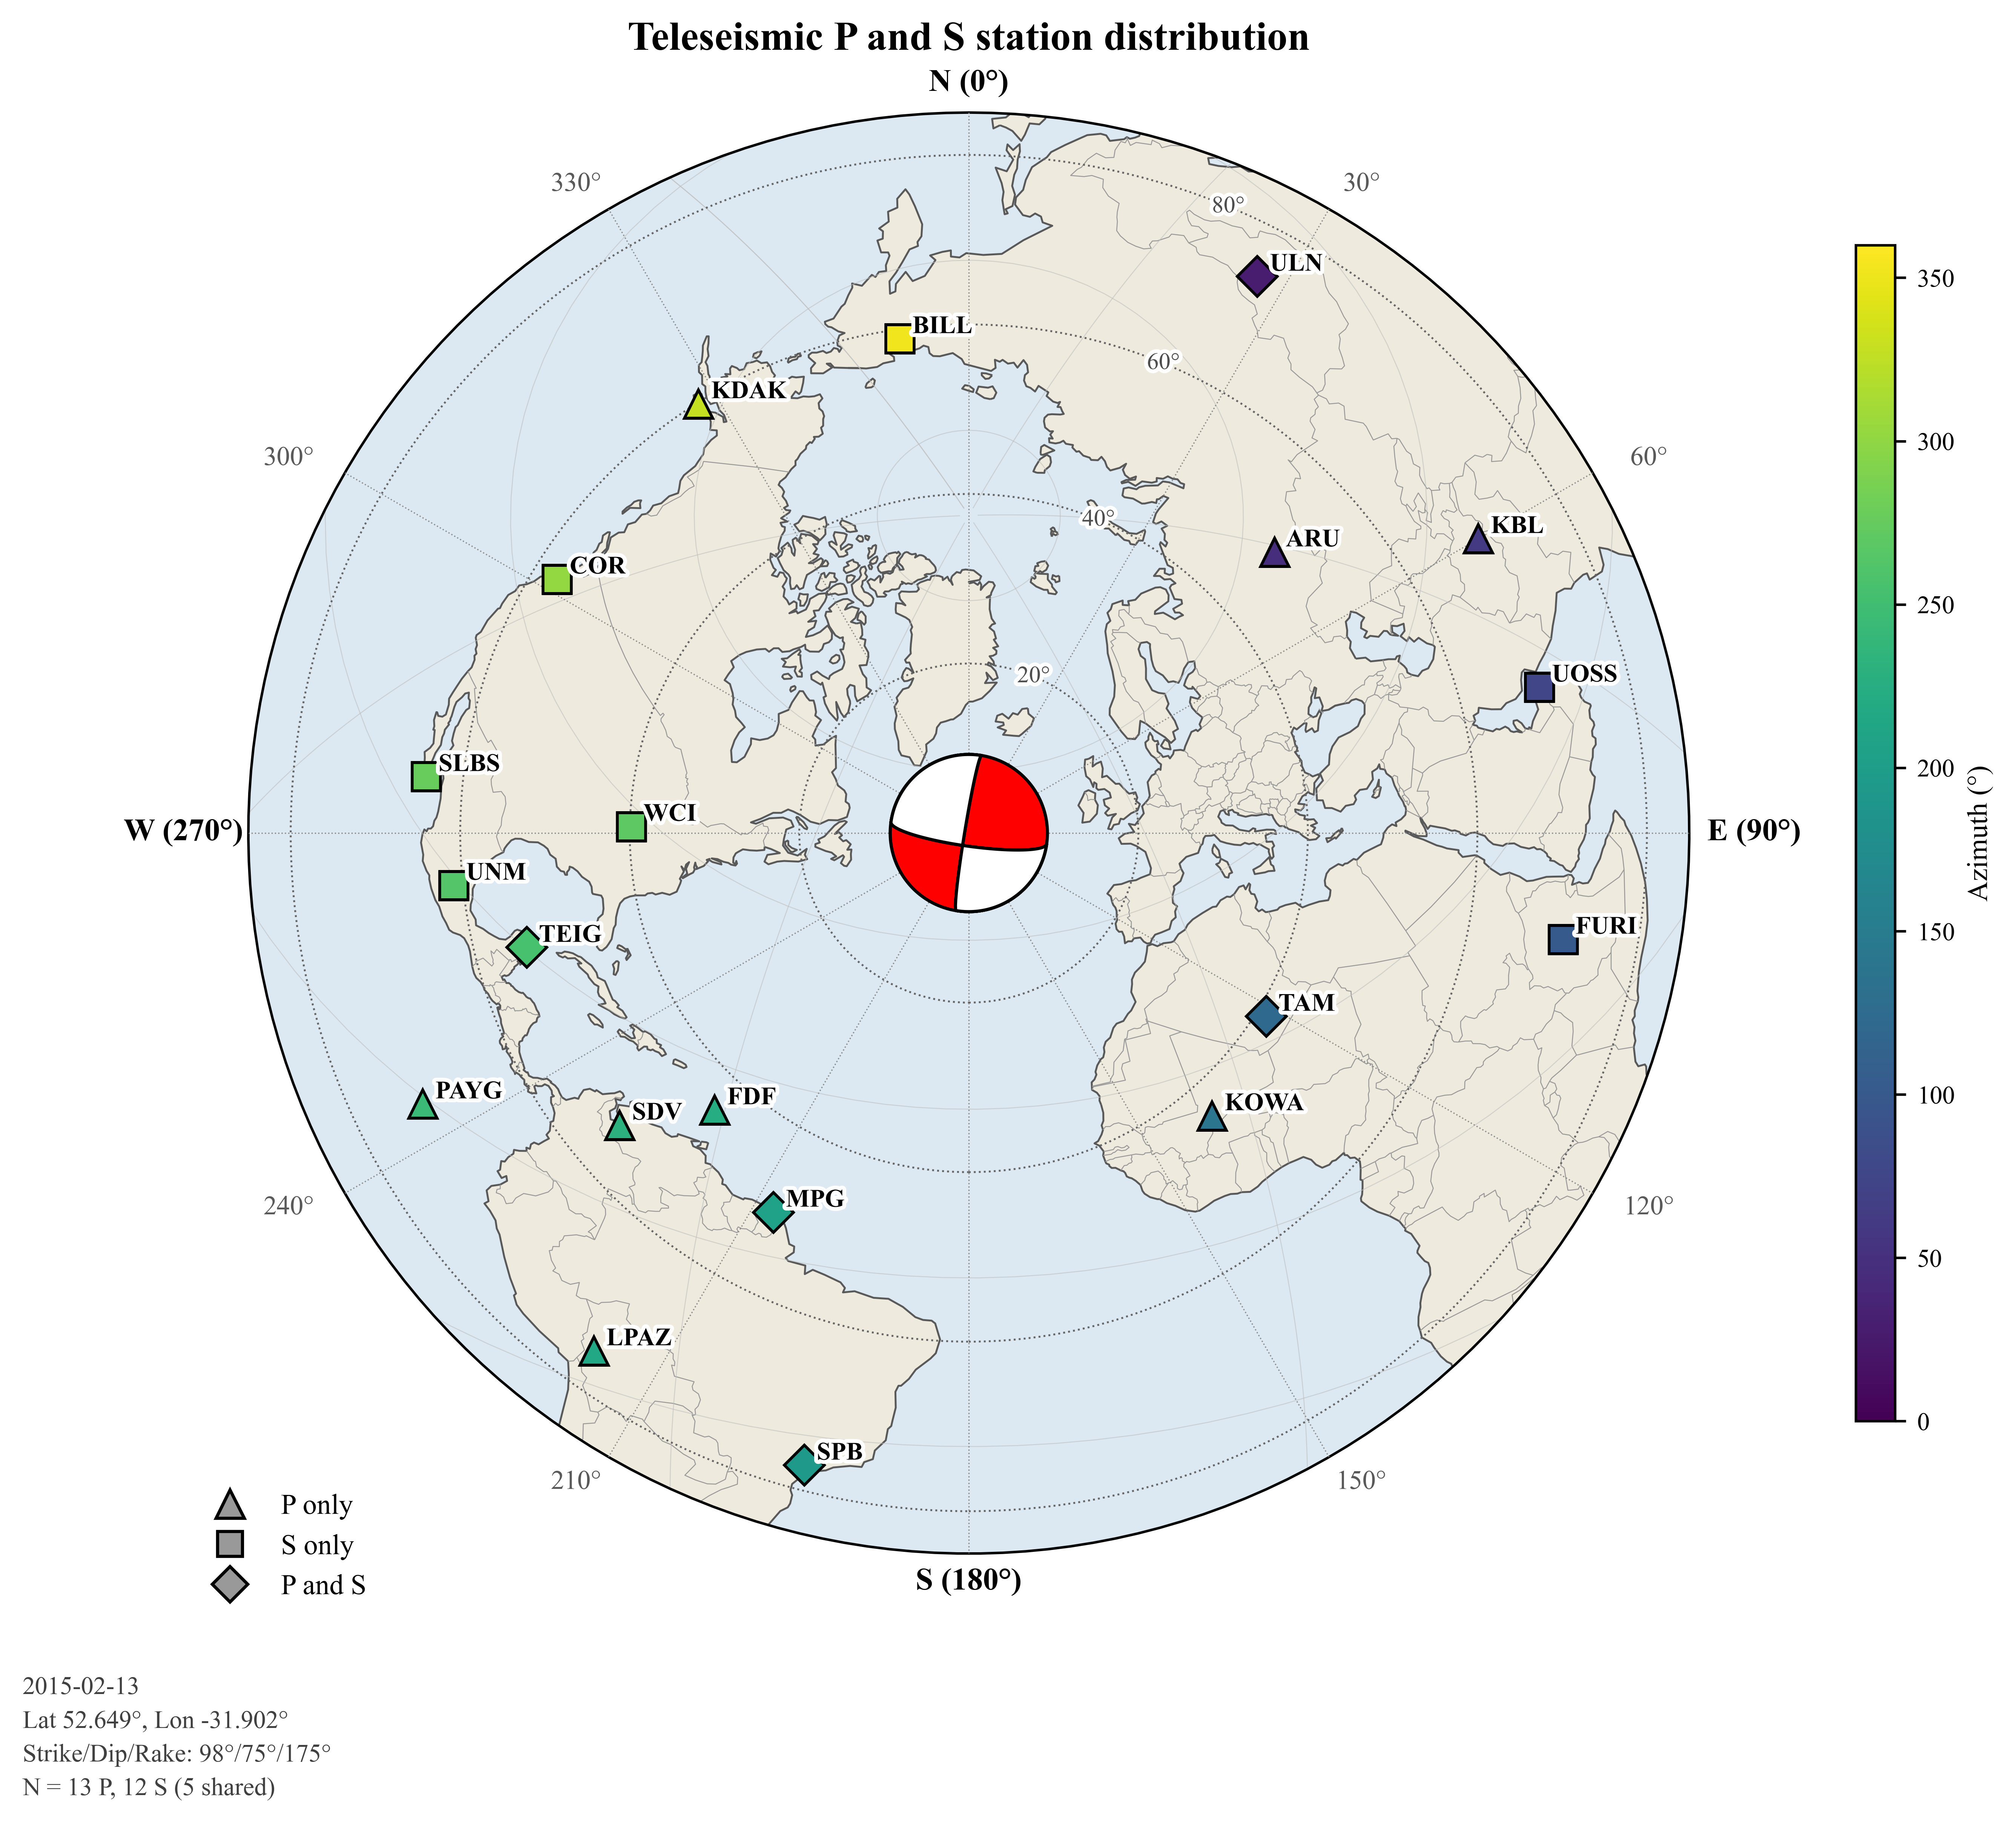
\includegraphics[width=\textwidth]{diagrams/2015_Charlie_Gibbs_P_S_station_distribution.png}
                \caption{}
                \label{fig:2015_tele_station}
            \end{subfigure}
            \hfill
            \begin{subfigure}{0.40\textwidth}
                \centering
                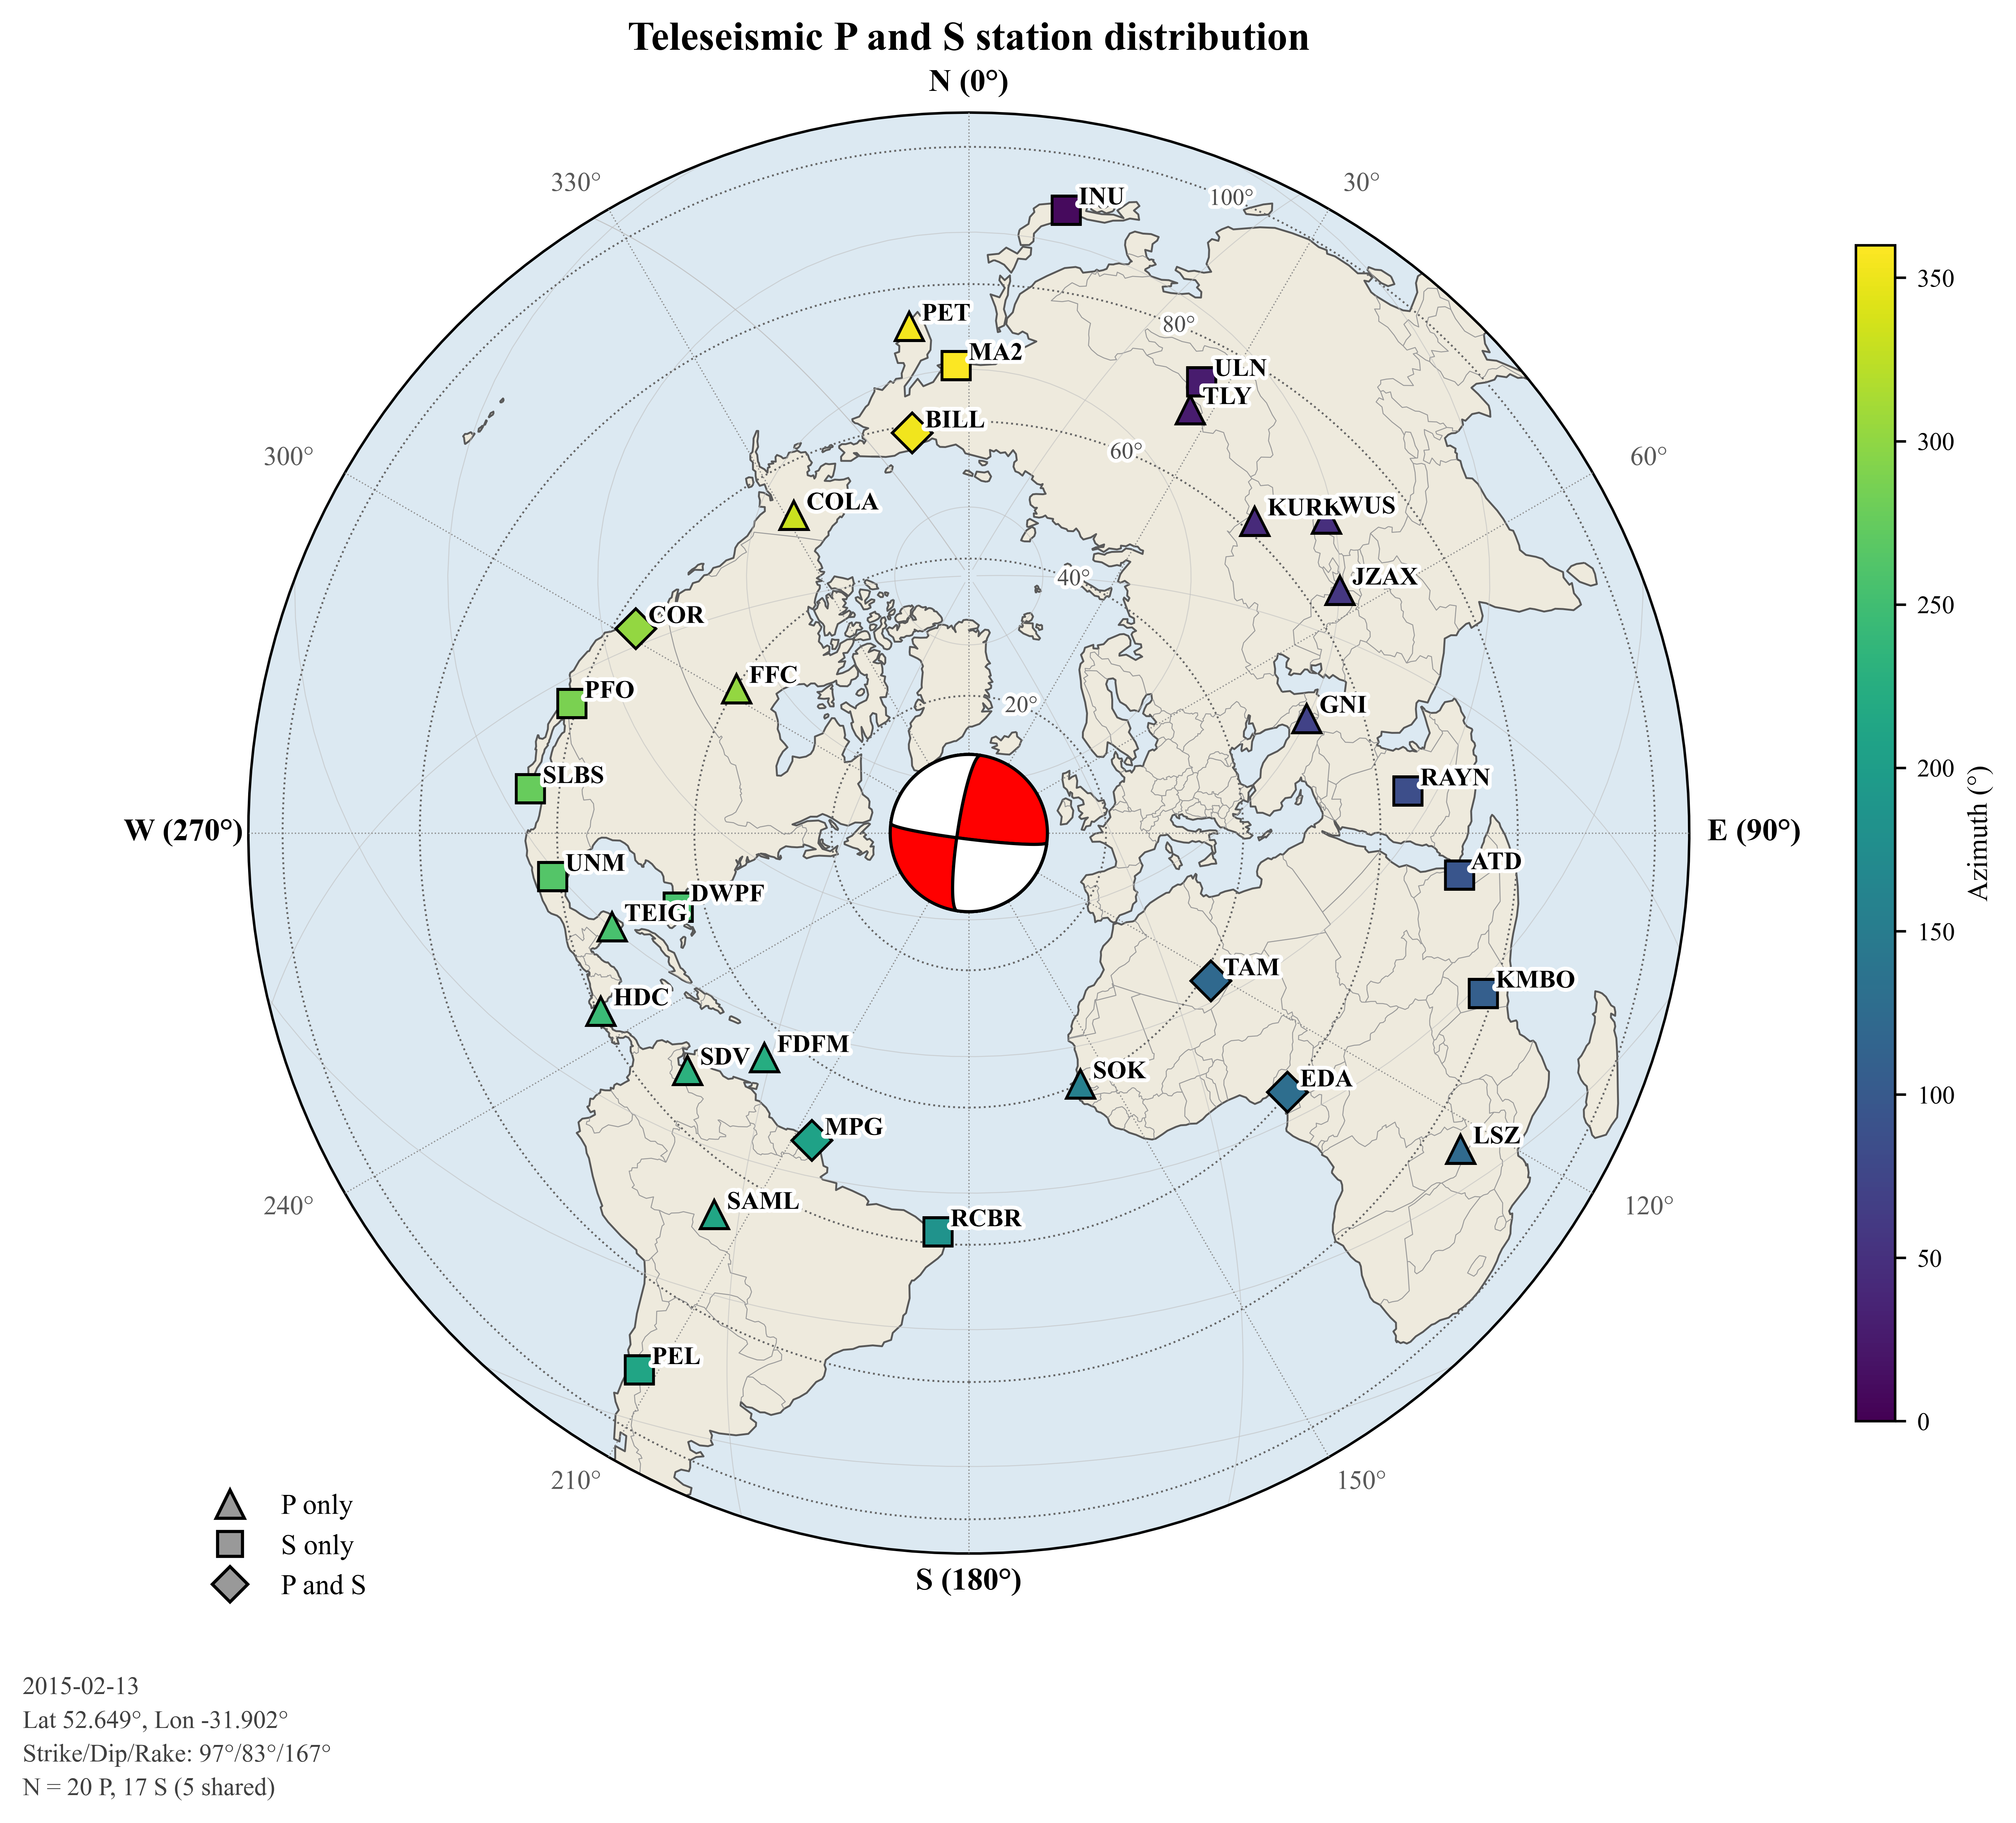
\includegraphics[width=\textwidth]{diagrams/2025_Charlie_Gibbs_P_S_station_distribution.png}
                \caption{}
                \label{fig:2025_tele_station}
            \end{subfigure}

            \vspace{0.2cm}

            % ---------- 2025 ----------
            \begin{subfigure}{0.38\textwidth}
                \centering
                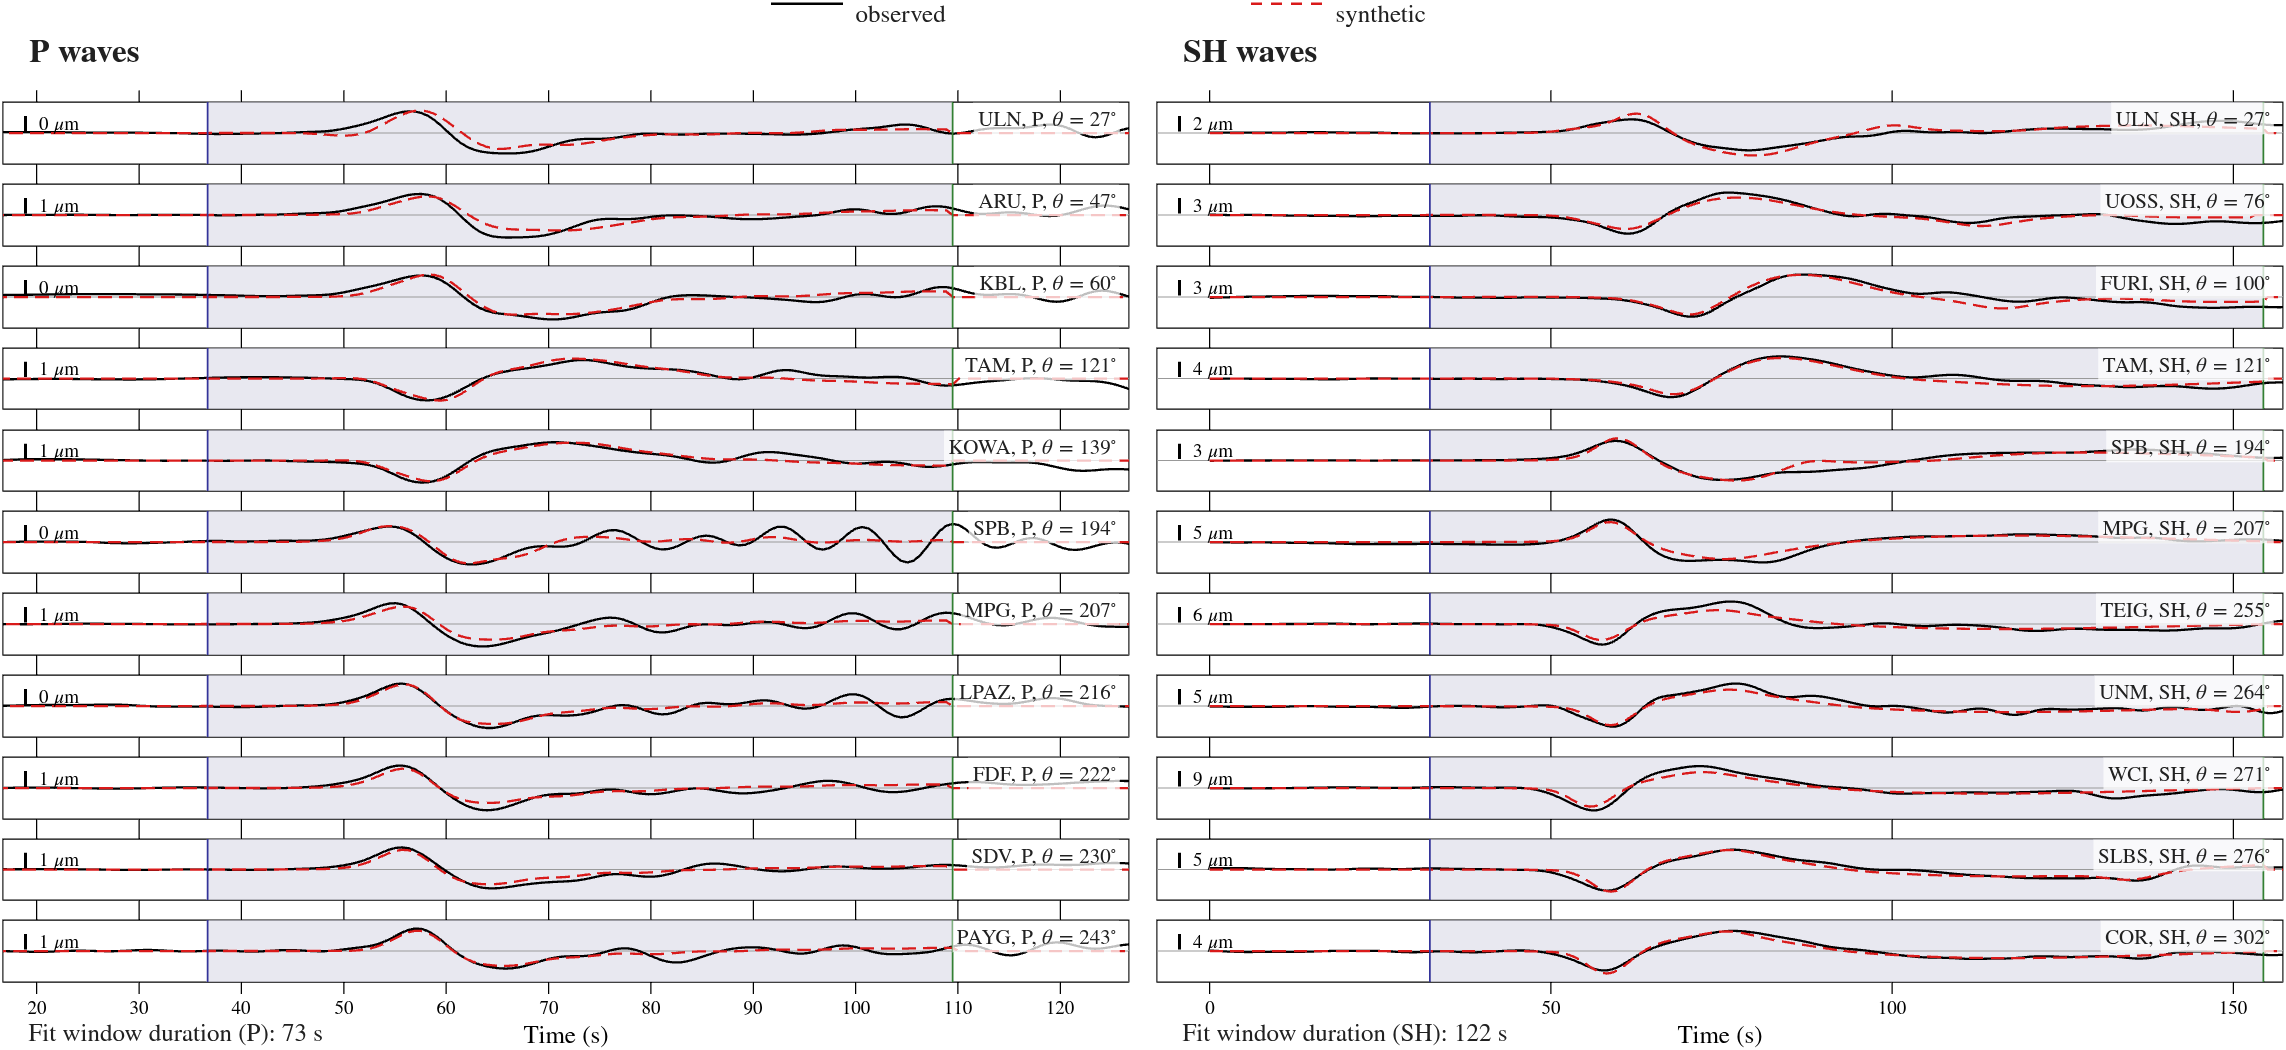
\includegraphics[width=\textwidth]{diagrams/2015_tele_inversion.png}
                \caption{}
                \label{fig:2015_tele_inversion}
            \end{subfigure}
            \hfill
            \begin{subfigure}{0.48\textwidth}
                \centering
                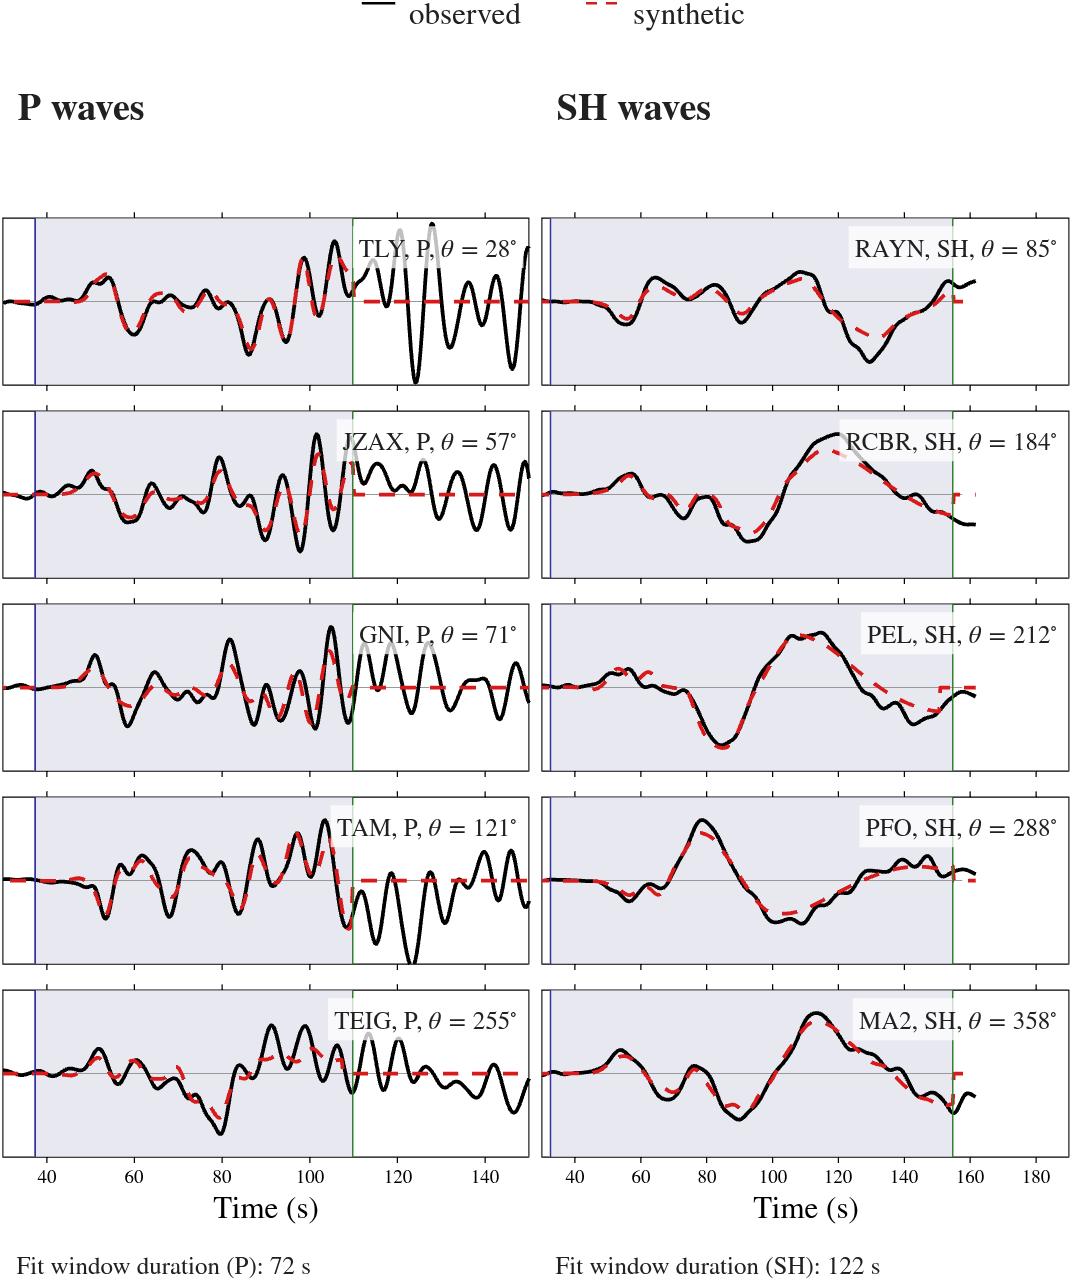
\includegraphics[width=\textwidth]{diagrams/2025_tele_inversion.png}
                \caption{}
                \label{fig:2025_tele_inversion}
            \end{subfigure}

        \end{minipage}%
    }

    \caption{Observed and synthetic teleseismic waveforms from deterministic wave modeling of the 2015 and 2025 Charlie–Gibbs 
    earthquakes as a part of joint inversion. (a) Distribution of teleseismic P- and S-wave stations used for the 2015 earthquake. 
    Triangles denote P-wave 
    stations, squares denote S-wave stations, and diamonds denote stations used for both P- and S-wave modeling. The color scale 
    represents epicentral distance. (b) Same as (a) for the 2025 earthquake. (c) Observed (black) and synthetic (red) P- and 
    SH-wave seismograms from deterministic wave modeling of the 2015 earthquake. Station names and azimuths ($\theta$) are indicated alongside
     the corresponding waveforms. (d) Same as (c) for the 2025 earthquake.}

    \label{fig:teleseismic_inversion}

\end{figure}


    \item And the RSTFs obtained from the inverted slip distribution also show good agreement too with the observed RSTFs, as shown
     in Figure~\ref{fig:rstf_inversion} having an aggregate rms of 0.126 for 2025 and 0.128 for 2015.

\begin{figure}[H]
    \centering

    \resizebox{0.9\textwidth}{!}{%
        \begin{minipage}{\textwidth}
            \centering

            % ---------- 2015 ----------
            \begin{subfigure}{0.48\textwidth}
                \centering
                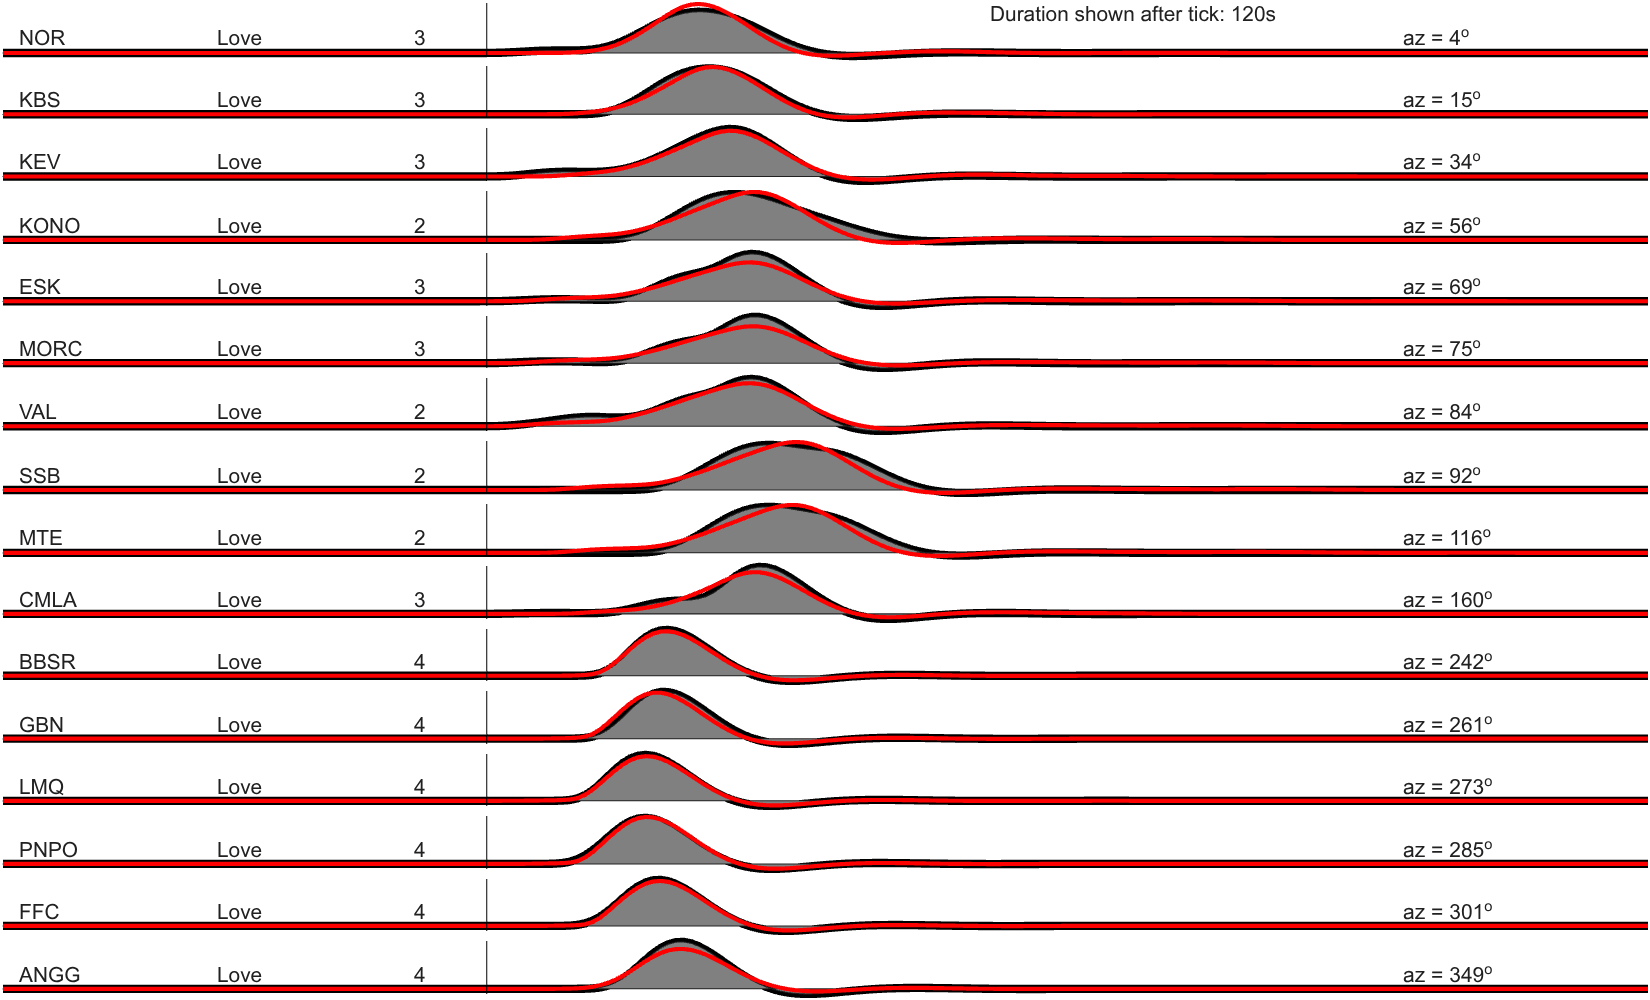
\includegraphics[width=\textwidth]{diagrams/2015_rstf_inversion.png}
                \caption{}
                \label{fig:2015_rstf_station}
            \end{subfigure}
            \hfill
            \begin{subfigure}{0.48\textwidth}
                \centering
                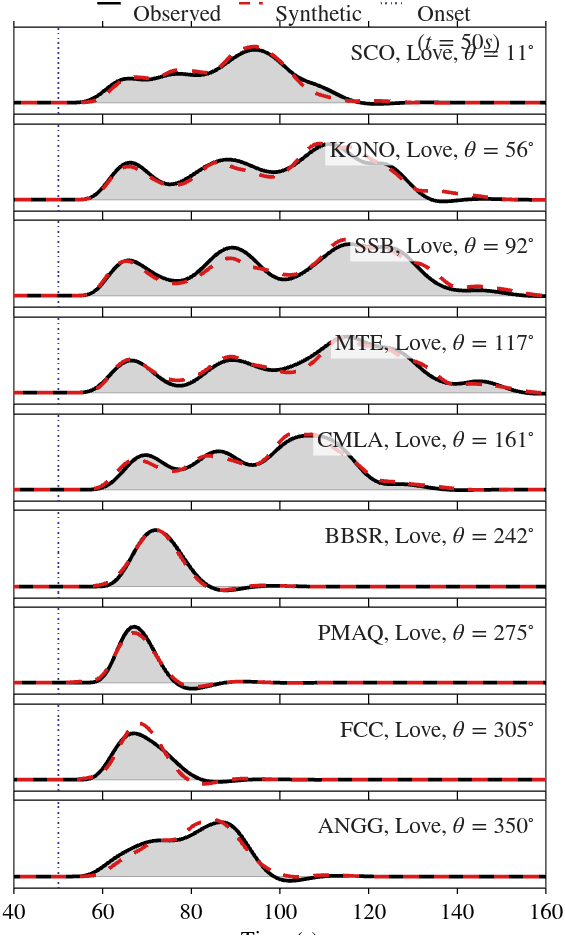
\includegraphics[width=\textwidth]{diagrams/2025_rstf_inversion.png}
                \caption{}
                \label{fig:2025_rstf_station}
            \end{subfigure}

        \end{minipage}%
    }

    \caption{Comparison between observed and synthetic relative source time functions (RSTFs) derived from Love-wave
     observations for the 2015 and 2025 Charlie--Gibbs earthquakes. (a) Observed (black) and synthetic (red) RSTFs for the 2015 
     earthquake, arranged according to station azimuth. Station names and azimuths ($\theta$) are indicated with the 
     corresponding RSTFs. (b) Same as (a) for the 2025 earthquake. The comparison between the observed and synthetic RSTFs shows the 
     fit from the inversion of the fault slip distribution, with an aggregate RMS misfit of 0.128 for the 2015 earthquake and 0.126 
     for the 2025 earthquake.}

    \label{fig:rstf_inversion}

\end{figure}
    \item The inverted slip distributions for the 2015 and 2025 earthquakes are shown in Figure~\ref{fig:slip_distribution_2015}\
     and Figure~\ref{fig:slip_distribution_2025}, respectively.The 2015 earthquake exhibits a concentrated slip distribution with 
     a maximum slip of 1.1~m, while the 2025 earthquake shows 
    a more distributed slip pattern with a maximum slip of 0.27~m. The total seismic moment released by the 2015 earthquake
    is $4.16 \times 10^{19}$~Nm, whereas the 2025 earthquake released $2.89 \times 10^{19}$~Nm. Our inversion found the average 
    rupture velocity of around 2.7 km/s for 2015 which is consistent with the findings of 2-4 km/s (\citeA{Aderhold2016}), and 
    3.1 km/s for 2025. These results indicate that the two earthquakes had different rupture characteristics, with the 2025 event
    being more spatially extended and having a longer duration than the 2015 event.
    \item The comparison of the retrieved source time functions shows the differences in the rupture duration and moment release between the two earthquakes. The 2015
     earthquake had a rupture duration of about 35 seconds with a strong peak in moment rate. In contrast the 2025 earthquake released
      moment at a lower amplitude but over a longer period lasting around 60 seconds. These patterns highlight rupture behaviors, 
      between the two events. STFs are shown in Figure~\ref{fig:stf_comparison}.
\begin{figure}[H]
    \centering
    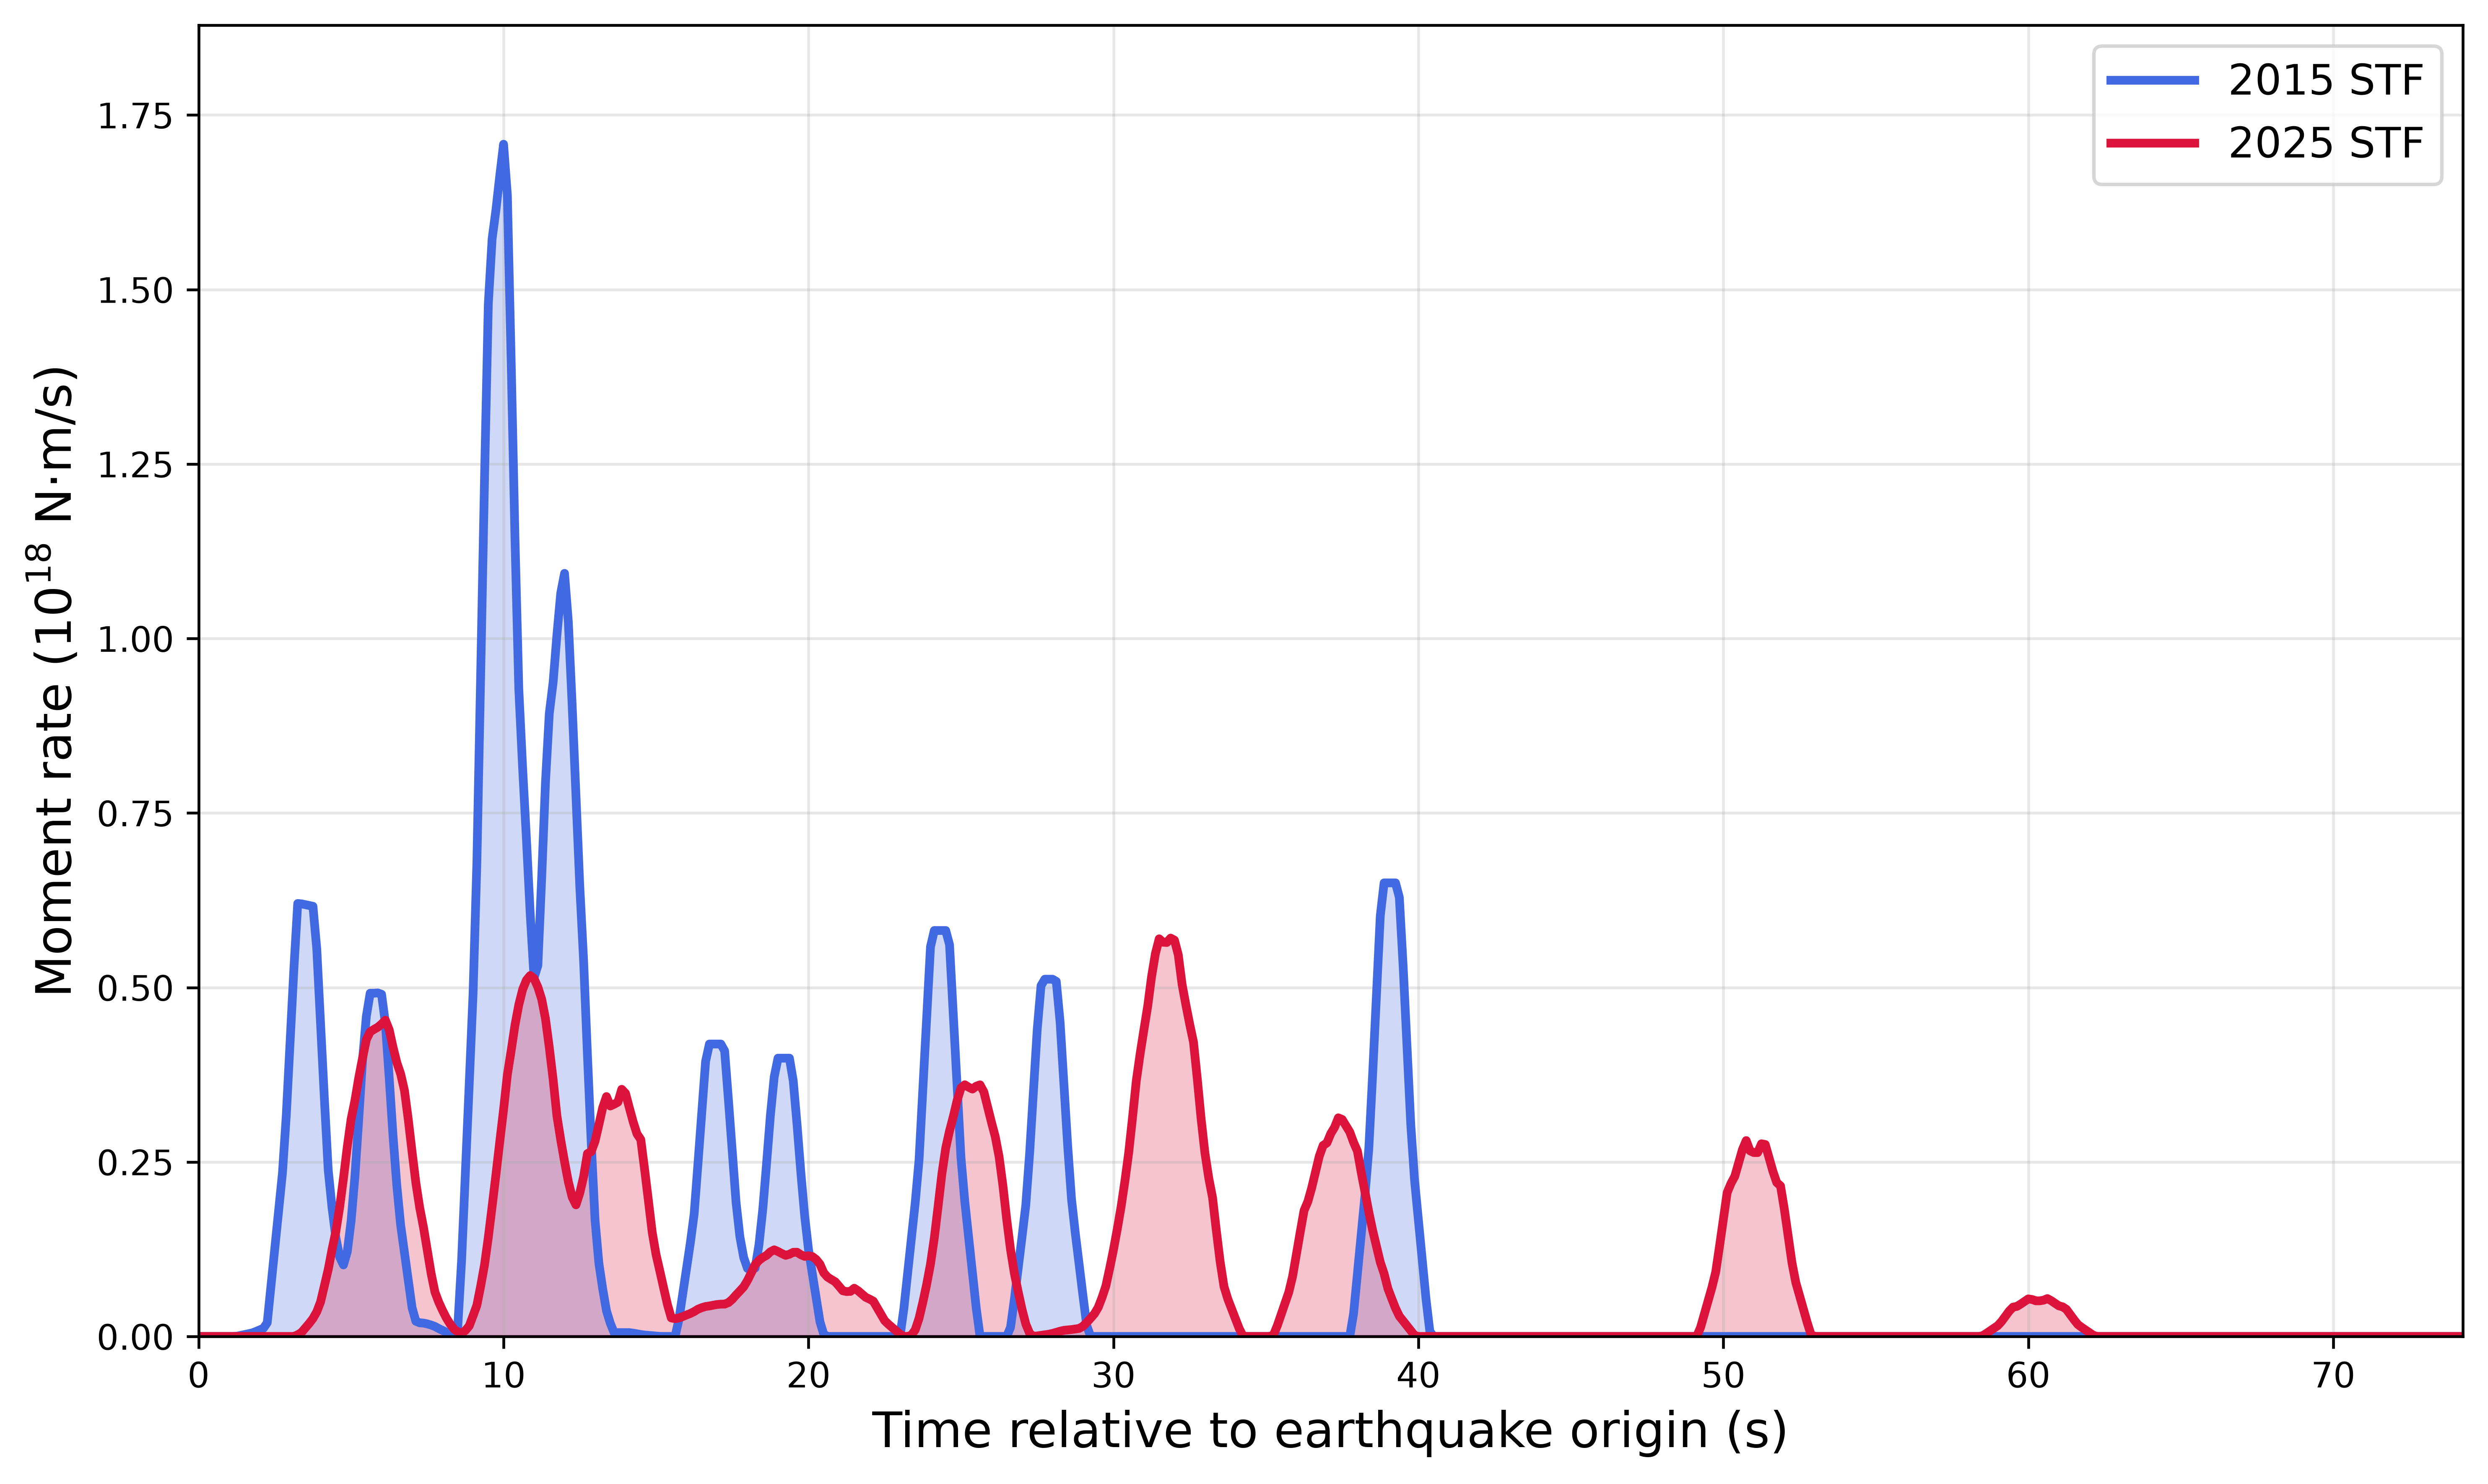
\includegraphics[width=0.7\textwidth]{diagrams/stf_comparison.png}
    \caption{Comparison of the source-time functions for the 2015 and 2025 Charlie--Gibbs earthquakes. 
    The blue and red curves show the moment-rate functions for the 2015 and 2025 earthquakes, respectively. The 2015 earthquake
     has most of its moment release concentrated within the first $\sim$30~s, whereas the 2025 earthquake exhibits moment release
      over a longer time interval, extending to approximately 60~s.}
    \label{fig:stf_comparison}
\end{figure}

    \item The rake distribution for both earthquakes is shown in Figure~\ref{fig:slip_distribution_2015} and 
        Figure~\ref{fig:slip_distribution_2025}. Both earthquakes show similar rake patterns towards west direction with average 
        rake amount of 175° and 184° for the 2015 and 2025 earthquakes, respectively.
\begin{figure}[H]
    \centering
    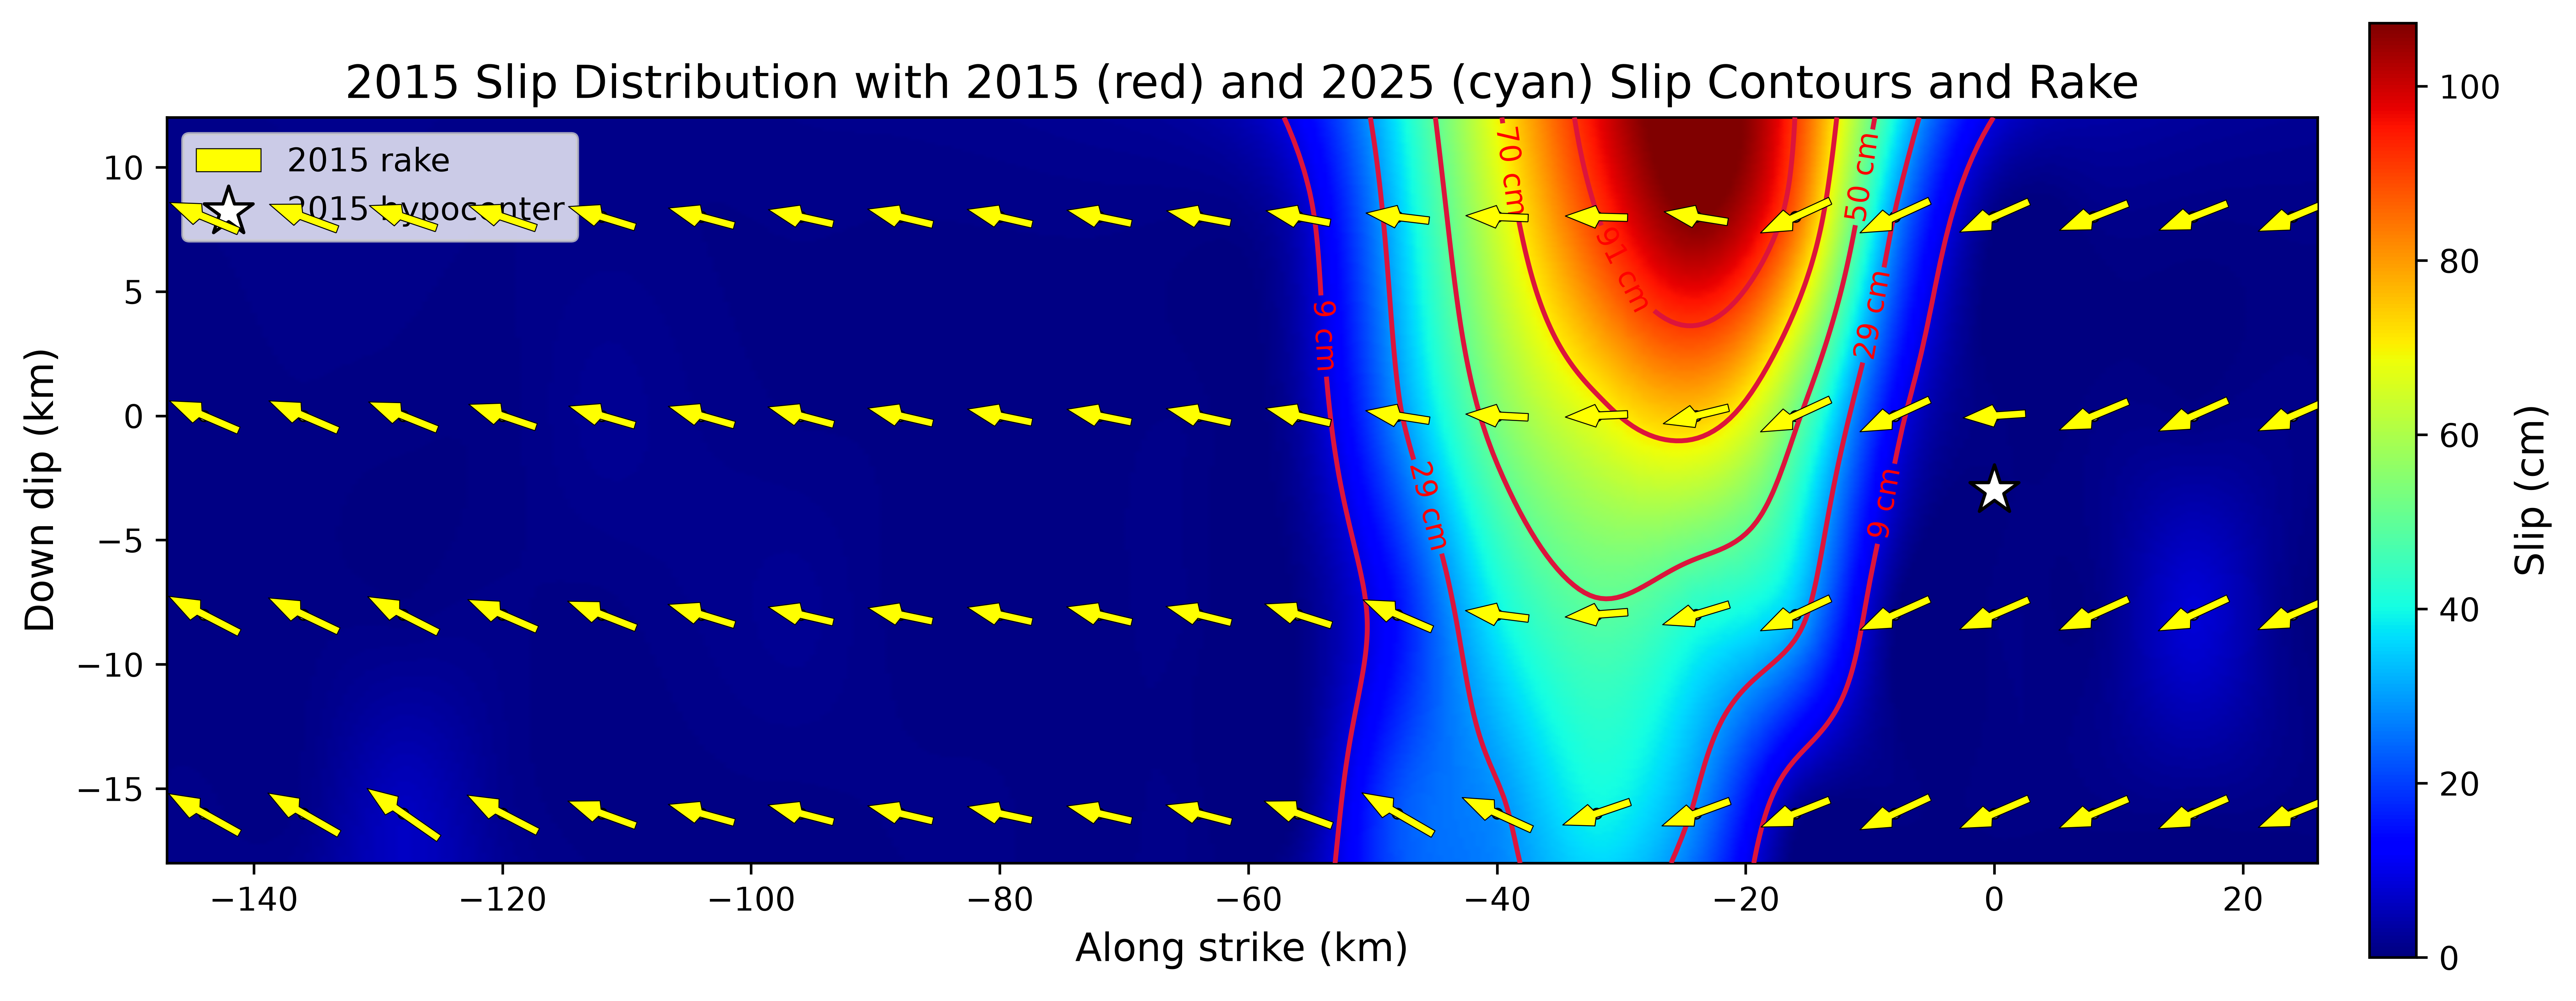
\includegraphics[width=0.9\textwidth]{diagrams/slip_rake_2015.png}
    \caption{Inverted slip distribution for the 2015 Charlie--Gibbs earthquake. The color scale represents the estimated slip
     amplitude with maximum slip of 1.1m, while the yellow arrows indicate the rake direction across the fault plane. 
     The star marks the hypocenter. Red contours show the slip distribution with slip values starting from 9cm.}
    \label{fig:slip_distribution_2015}
\end{figure}
\begin{figure}[H]
    \centering
    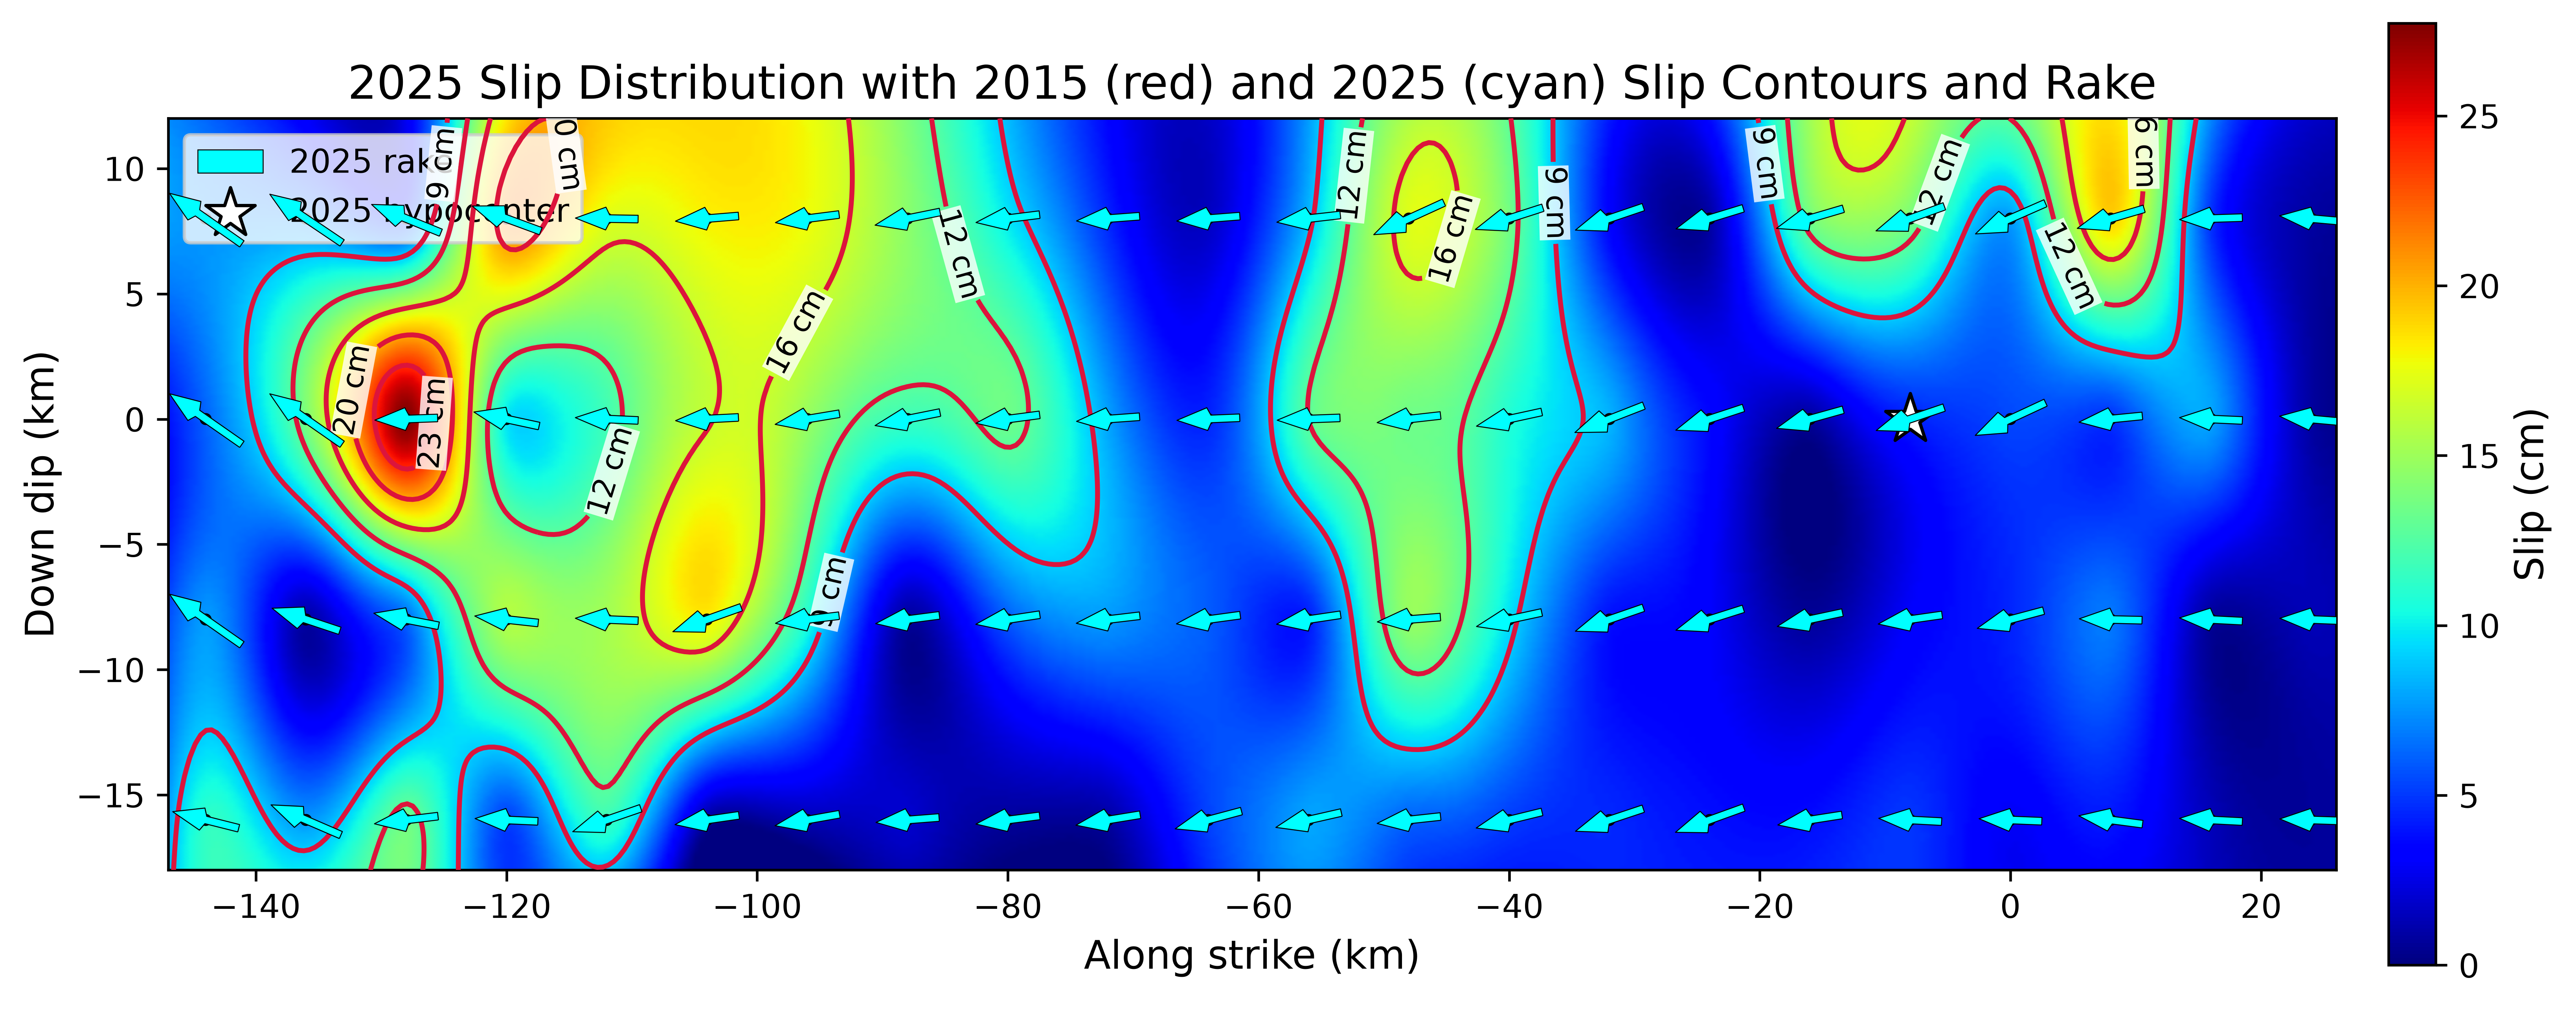
\includegraphics[width=0.9\textwidth]{diagrams/slip_rake_2025.png}
    \caption{Inverted slip distribution for the 2025 Charlie--Gibbs earthquake. The color scale represents the estimated slip
     amplitude with maximum slip of 0.27m, while the cyan arrows indicate the rake direction across the fault plane. 
     The star marks the hypocenter. Red contours show the slip distribution with slip values starting from 9cm.}
    \label{fig:slip_distribution_2025}
\end{figure}

    \item The 2015 earthquake shows a relatively concentrated slip distribution, with the main asperity confined to the 0- -60~km (Figure~\ref{fig:slip_distribution_2015})
     section along strike. In contrast, the 2025 earthquake exhibits a more distributed slip pattern with multiple asperities. 
     One asperity is located around $-20$ to $+20$~km along strike, a second extends from approximately $-30$ to $-60$~km, while 
     a third occupies the western section of the fault, extending from approximately $-70$ to $-148$~km (Figure~\ref{fig:slip_distribution_2025}).

     \item To investigate the relationship between the slip distributions of the two earthquakes, we compared the slip contours of 
     both events in a single figure (Figure~\ref{fig:slip_contours_2015_2025}). It seen observed that in the region where most of the 
     2015 slip occurred, the 2025 earthquake shows low to no slip suggesting that the 2015 slip asperity may have released the 
     accumulated stress in that region which did not have enough time to re-accumulate before the 2025 earthquake occurred.
     But there are also some overlapping regions which can be result of dynamic stress transfer from 2015 earthquake.
     But it was out of the scope of this study to investigate the stress transfer and stress accumulation along the fault system but 
     can be investigated in future studies. 
     \item We also tried to model dip as we kept dip as a free parameter in the inversion and this improved our model fit to the data.
     Inversion results from fixed dip is shown in the supplementary material. 
\begin{figure}[H]
    \centering
    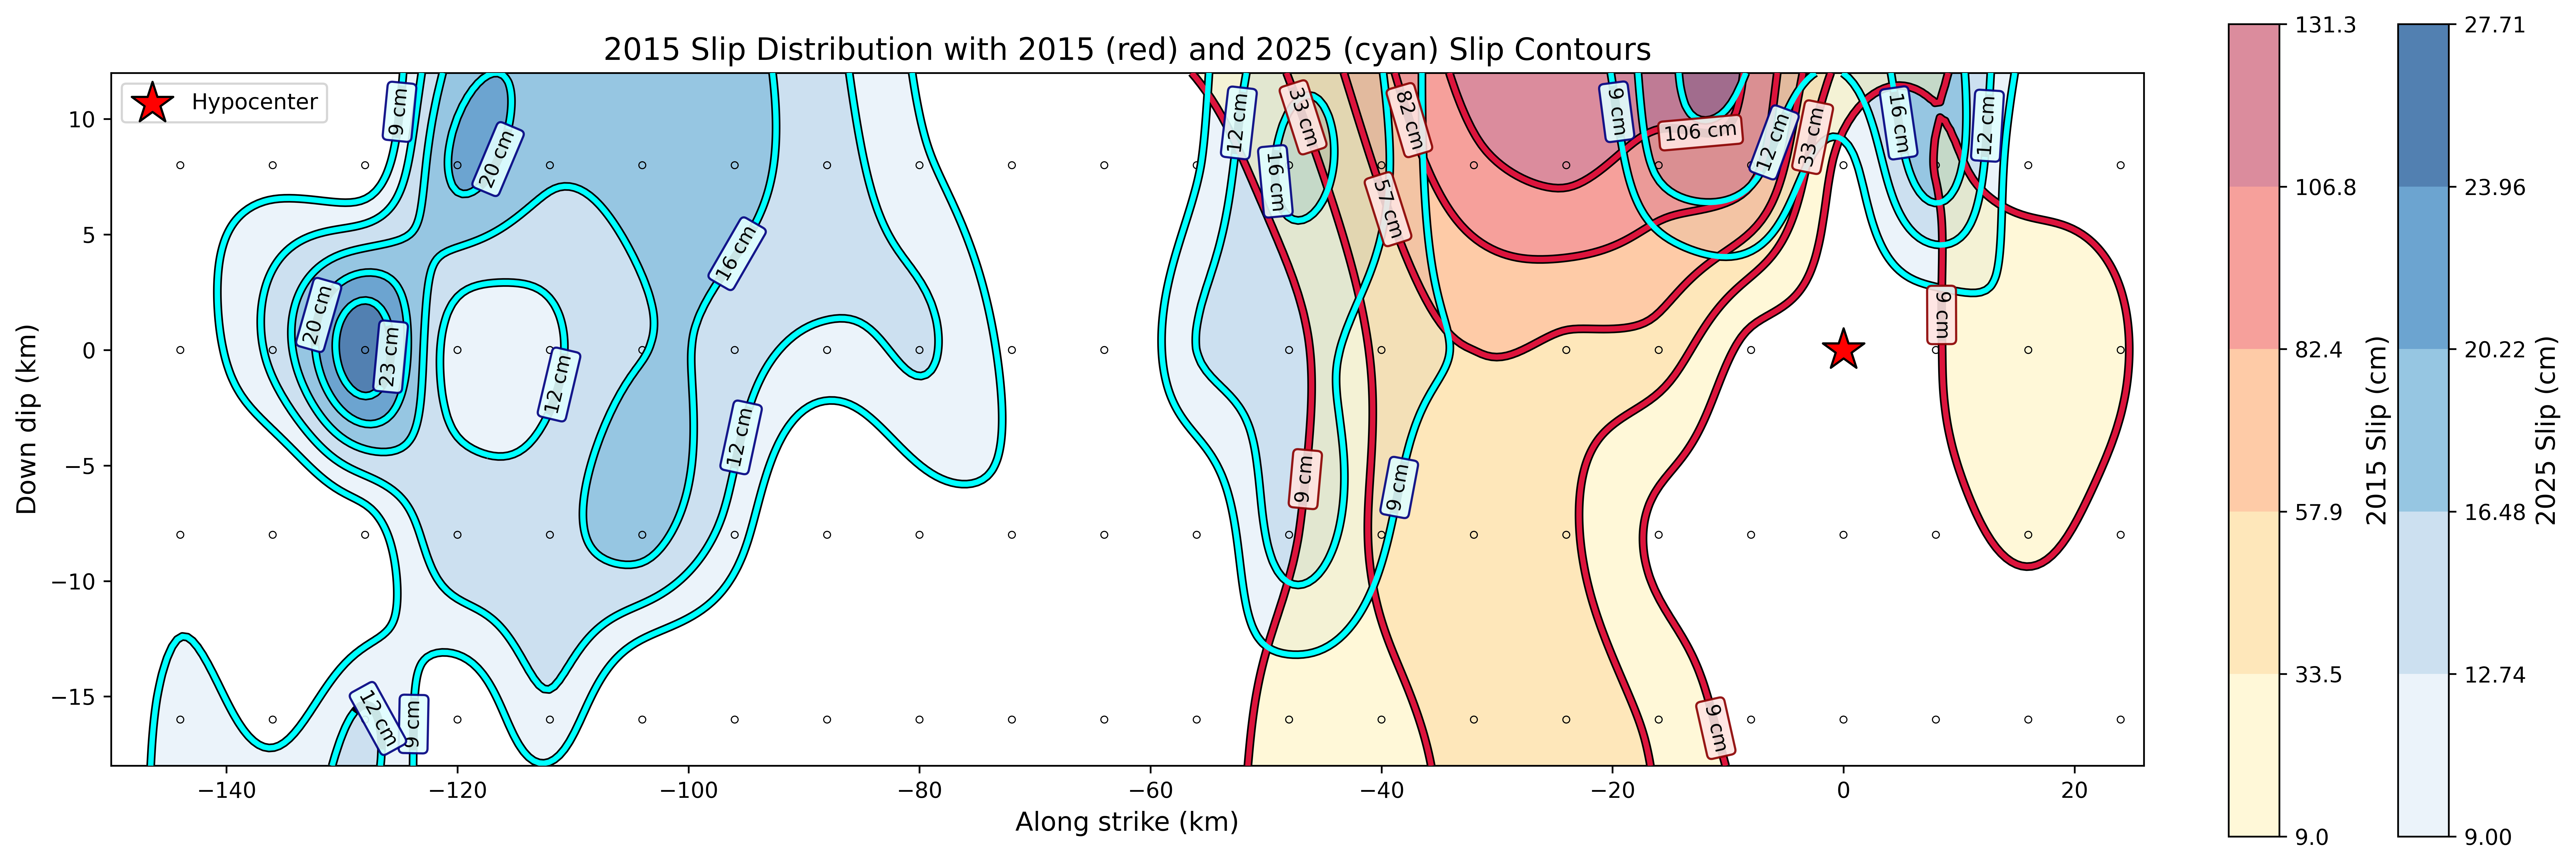
\includegraphics[width=0.9\textwidth]{diagrams/slip_contours_2015_2025.png}
    \caption{Comparison of the inverted slip distributions for the 2015 and 2025 Charlie--Gibbs earthquakes on the same fault geometry. 
    The color-filled distribution represents the 2015 slip amplitude, with red contours showing the 2015 slip distribution and cyan
     contours showing the 2025 slip distribution. Red and cyan stars mark the hypocenters of the 2015 and 2025 earthquakes, respectively.
      The horizontal and vertical axes represent distance along strike and down dip, respectively.}
    \label{fig:slip_contours_2015_2025}
\end{figure}

\end{itemize}